\section{Introduction}
The external features of an arthropod, \textit{i.e.}, the phenotypes we can easily observe through a microscope, are the primary source of characters we use to diagnose arthropods to higher-level taxonomic groupings. These phenotypes also inform us about natural history and inspire hypotheses of evolutionary relationships. Given the extraordinary diversity of Arthropoda, however, which includes well over 1,000,000 species, the lexicon entomologists use to refer to anatomical structures (and even to describe their form) is large, convoluted, and rich in homonyms and synonyms. Just look at the illustration below, from 1905 and published by Rev. W. J. Wingate \citeyearpar{wingate1906}. Recognize any of those terms?

\begin{figure}[ht!]
  \centering
    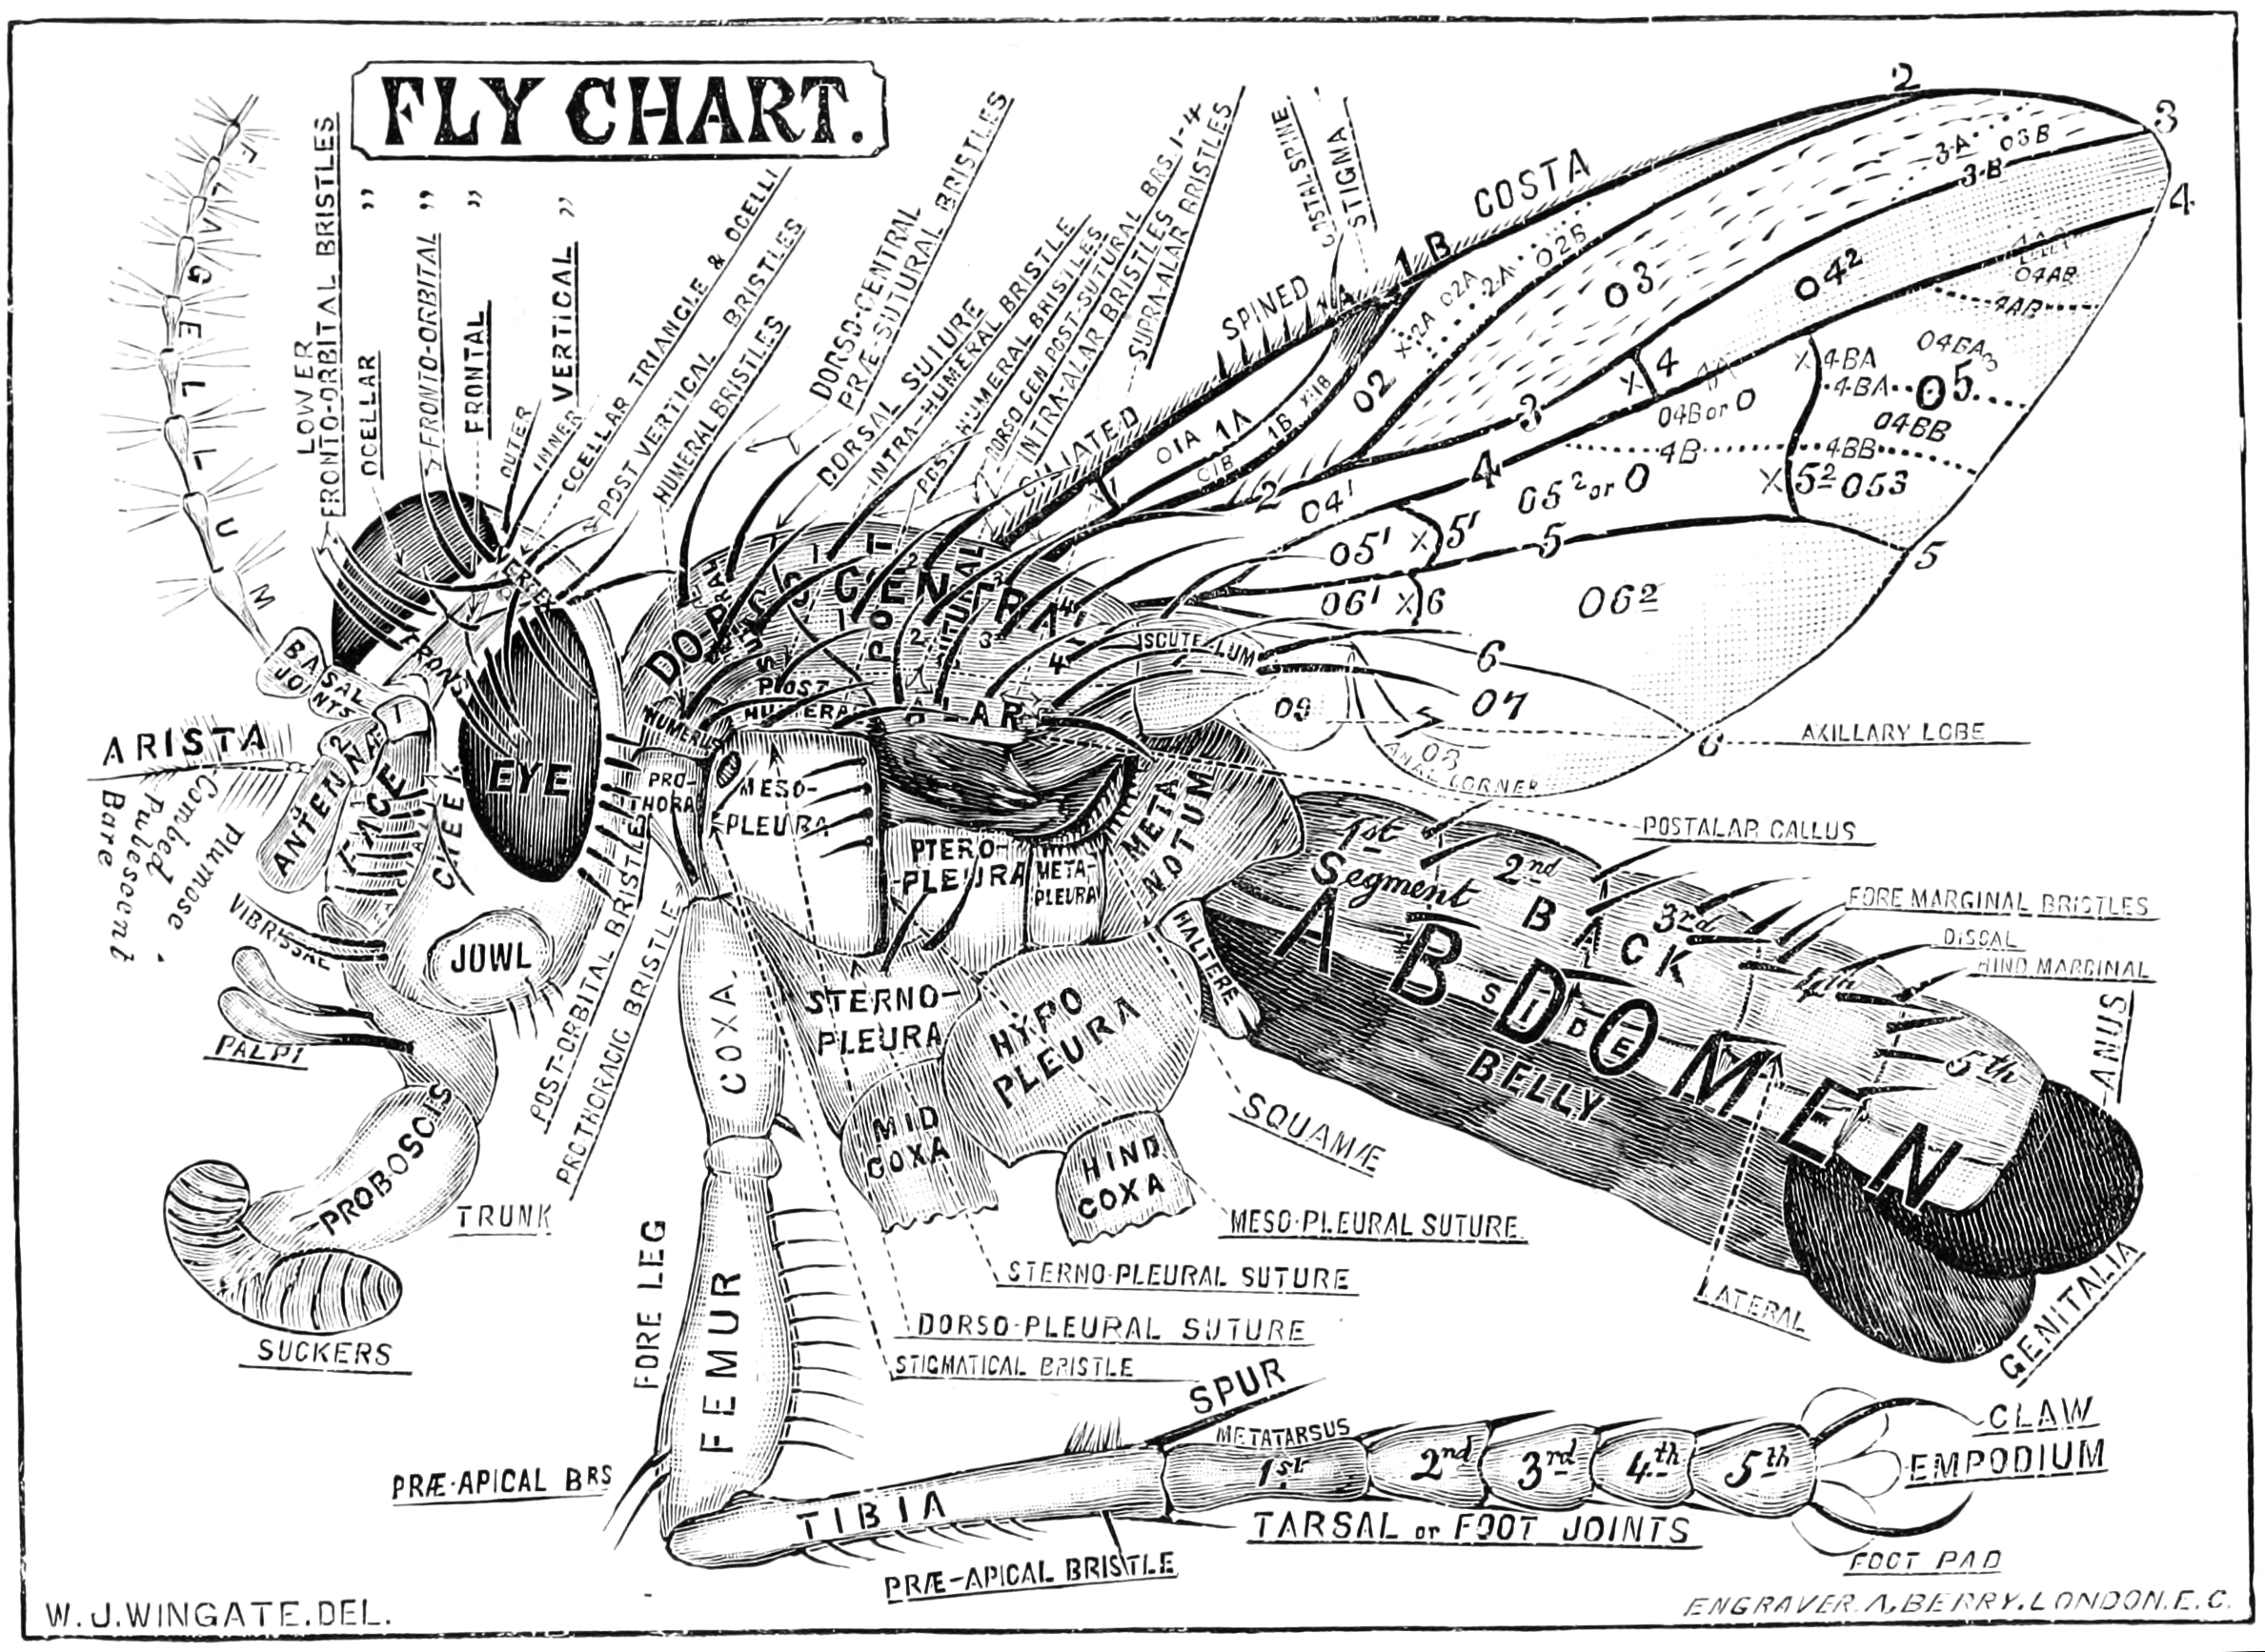
\includegraphics[width=0.84\textwidth]{morphology/flyAnatomy}
  \label{fig:flyAnatomy}
\end{figure}

In this lab we will observe specimens from across the phylogeny of Arthropoda, with an emphasis on Insecta. The goal is to familiarize yourself with the anatomical concepts relevant to most diagnostic keys and phylogenetic studies and to learn the various terms applied to these structures. Terms you should be comfortable with are differentiated by this \latinword{font}.

There is no single, perfect reference for insect anatomy and function. The treatise by \cite{snodgrass1935principles}, however, is a tested classic, which, despite being quite out of date regarding evolutionary hypotheses, covers most of the anatomy relevant to taxonomy. \cite{beutel2013insect} is a more contemporary treatment of insect morphology, with an emphasis on the phenotypes most relevant to our understanding of hexapod relationships.

\section{Methods}
Working with a partner, organize your space, specimens, tools, and microscope. Probes and forceps are available to manipulate the specimens. Some specimens may be available for dissection and more destructive observation; these will be clearly labeled (\textit{i.e.}, don't assume you can dissect just any specimen). Annotate the figures below and draw as many parts as possible in your notebook, from many different kinds of arthropods. Learn the \latinword{highlighted} words and be prepared to define them on an exam.

\section{Orientation}
Before we start looking at specific body parts take a few minutes to observe the specimens before you. Manipulate them with your forceps and probe under the microscope. Take some time to understand the biospatial concepts: \latinword{anterior}, \latinword{posterior}, \latinword{dorsal}, \latinword{ventral}, \latinword{lateral}, \latinword{proximal}, and \latinword{distal}. Label figure \ref{fig:biospatial} with these terms.\vspace{3mm}

\begin{figure}[ht!]
  \centering
    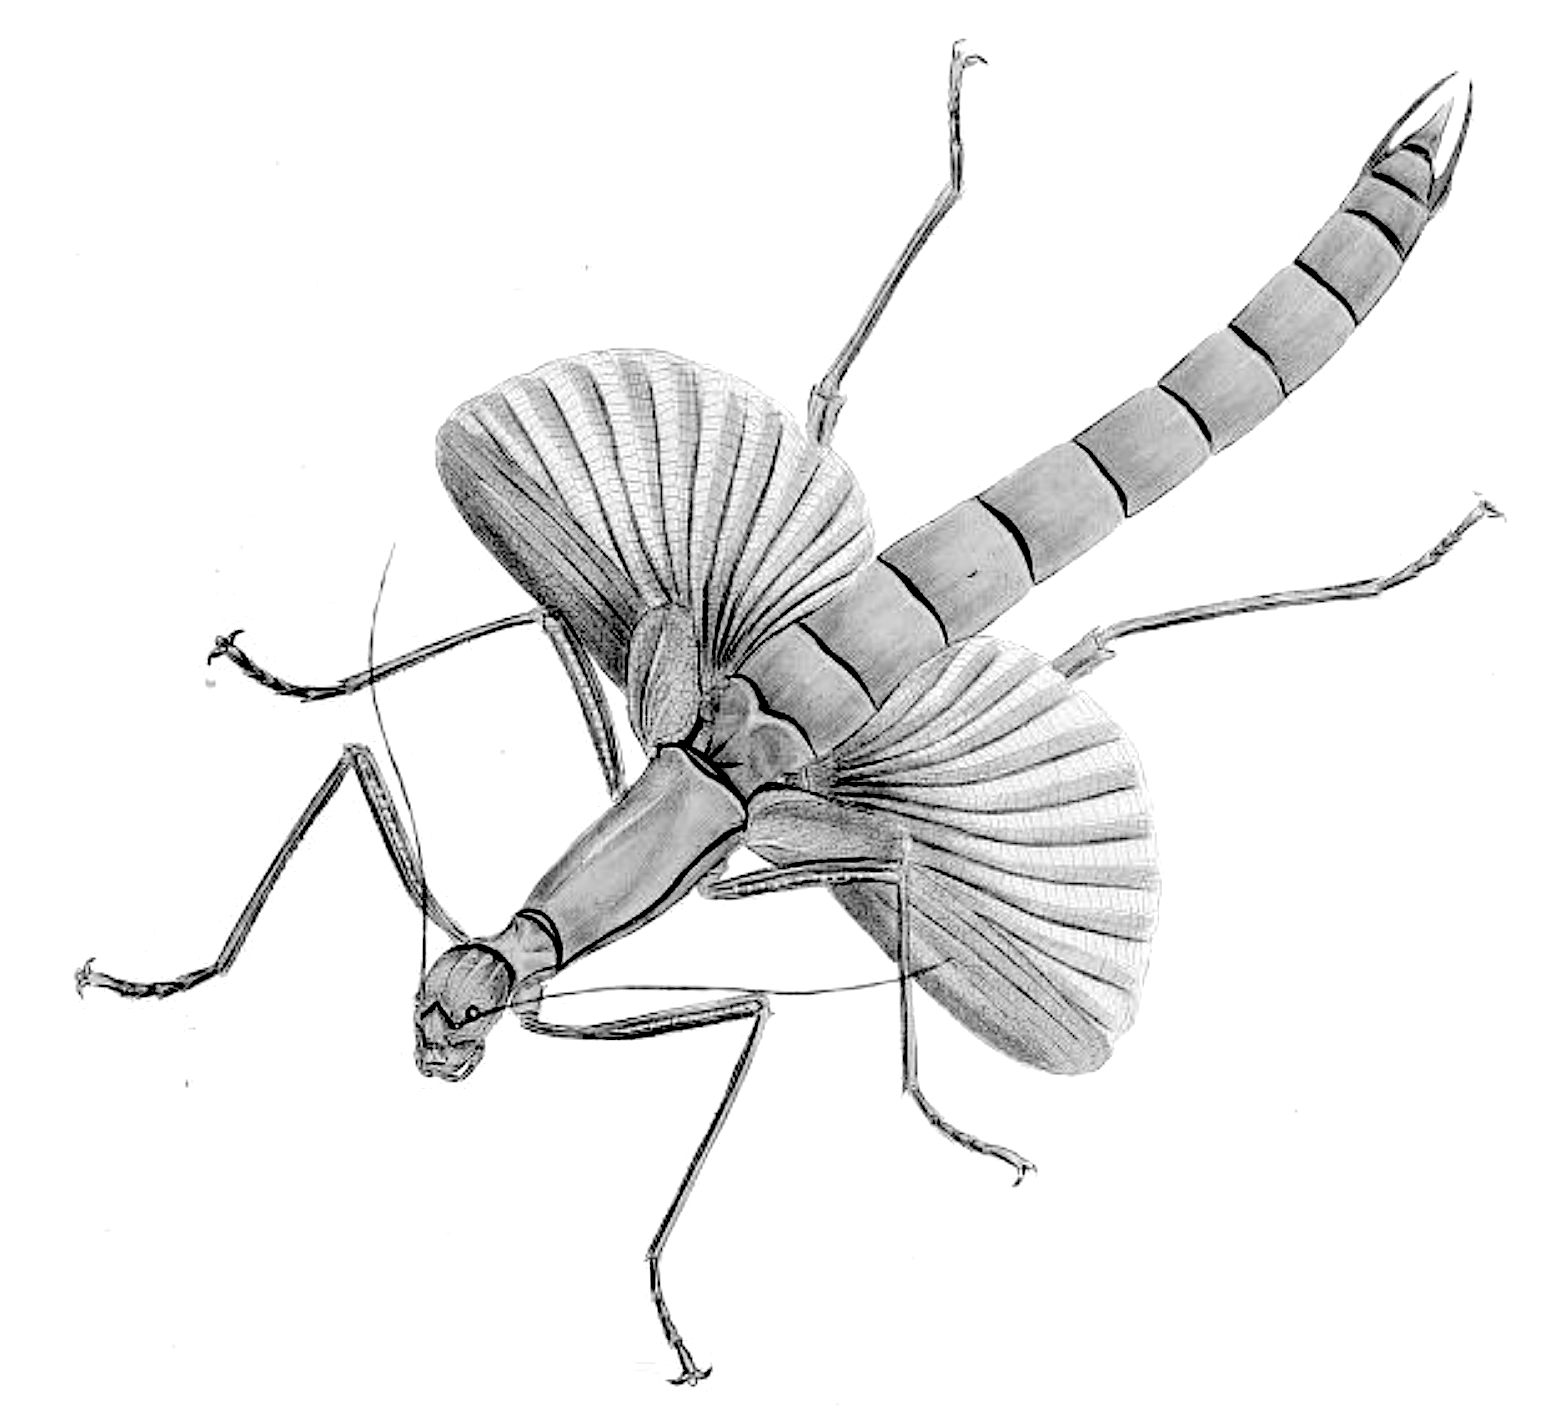
\includegraphics[width=0.55\textwidth]{morphology/biospatial}
  \caption{Phasmatodea \citep[][Plate X]{bhlitem104661}}
  \label{fig:biospatial}
\end{figure}

\begin{theo}
{}Observe several specimens you think represent different branches of the arthropod tree---\textit{e.g.}, a spider, a millipede, a beetle, and a few others. Can you describe at least three traits these organisms have in common?
\end{theo}

\section{Segmentation}
\latinword{Segments} are \latinword{metameric} subdivisions of the body or of appendages. Some researchers use ``segment'' only for those metameric subdivisions that meet certain criteria, for example if they each have intrinsic musculature. Using your forceps and probe, try to expand and contract your arthropod specimens. Separate two \latinword{flagellomeres} (subdivisions of the apical segment of the \latinword{antenna}, the \latinword{flagellum}) and then the \latinword{pedicel} (the medial antennal segment) from the \latinword{scape} (proximal segment of the antenna) on one of the beetles.\vspace{3mm}

\noindent{}Try to separate two segments on the \latinword{abdomen} of a specimen. Observe the difference in stiffness between the \latinword{arthrodial membrane} and a \latinword{sclerite}. \vspace{3mm}

\noindent{}\latinword{Tagmata} (\latinword{tagma}, sing.) are body regions composed of several segments that function together for certain, specialized purposes.\vspace{3mm}

\begin{theo}[traits2]
{}How are appendage segments separated from each other? Keep in mind that the taxon name Arthropoda is derived from the Greek \textit{árthron}, ``joint'', and \textit{pous}, ``foot'', which together refer to their jointed legs.\vspace{3mm}

\noindent{}What components of the segment define the segment's boundaries? Arthrodial membrane is much more flexible than sclerites; why do insects and other arthropods need soft cuticle? Can you find and count the tagmata on different specimens? Compare an insect to a spider and a harvestman.
\end{theo}

\begin{figure}[ht!]
  \centering
    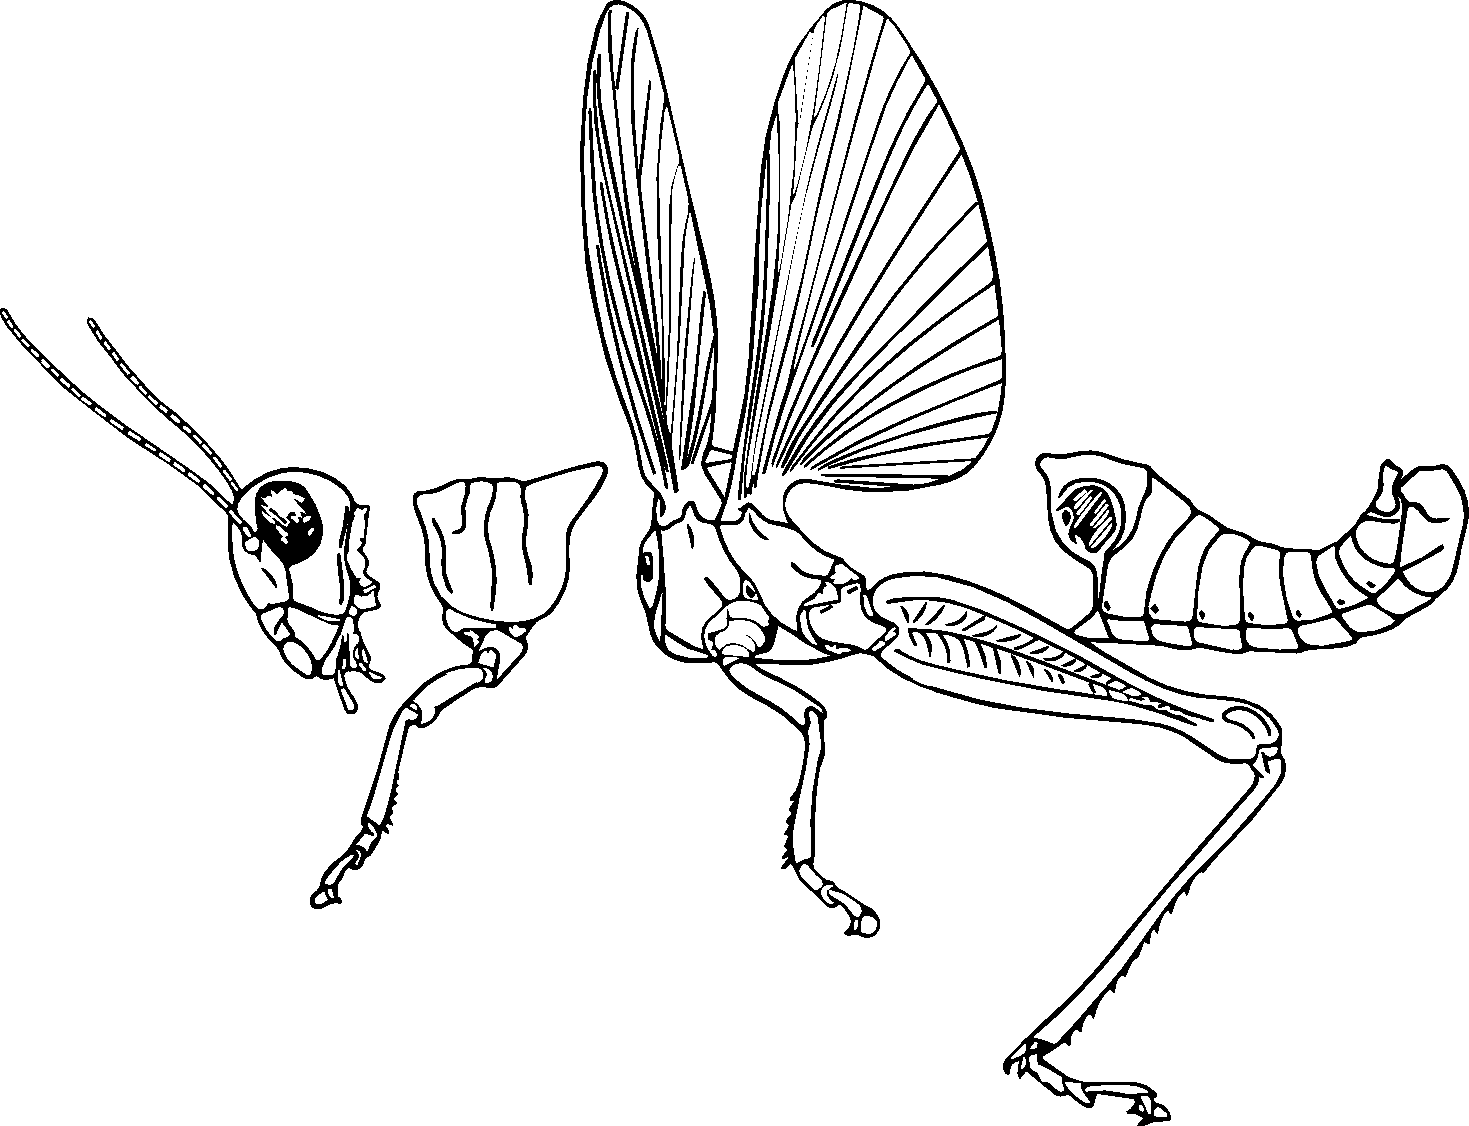
\includegraphics[width=0.7\textwidth]{morphology/Tagmata}
  \caption{Grasshopper. \citep[redrawn from ][Fig. 63]{bhl128276}}
  \label{fig:tagmata}
\end{figure}

\section{Appendages}
Each segment has \latinword{appendages} associated with it, at least ancestrally. Take a minute to familiarize yourself with the components of an appendage. \vspace{3mm}

\begin{theo}[appendage]
{}How would you define ``appendage''? Are wings appendages?
\end{theo}

\section{Head}
The first tagma we'll look at is the \latinword{head}. Spend some time examining the heads of your specimens, both of insects and of non-insects. Note the number and location of appendages and look for evidence of segmentation. \vspace{3mm}

\begin{theo}[traits3]
{}Compare multiple insect heads. How many segments comprise the head? Now look at the spider and harvestman. Do non-insect arthropods have the same head configuration as Insecta? What are the major functions of the head?
\end{theo}

\noindent{}The \latinword{antenna} is the most obvious metameric appendage of the head. As we have seen earlier, the flagellum of the insect antenna is not musculated (only the first two sclerites, the scape and the pedicel, which are true \latinword{appendage segments}, have muscle attachments). Some non-insect hexapods (like Collembola) and non-hexapod pancrustaceans have fully musculated antennae.\vspace{3mm}

\begin{theo}
{}How many antennae do insects have? What about spiders and crayfish? Some arthropods do not have antennae, while others have highly reduced antennae. How do these arthropods, like harvestmen (Opiliones), compensate for the lack of this useful structure? Why don't insects need a muscular flagellum? You observe different antenna phenotypes in your specimens. Why are antennae so diverse in shape?
\end{theo}

\noindent{}Let's focus on mouthparts, which are comprised of the other head appendages. When examining the insects in front of you, try to identify the following structures (figure \ref{fig:headCockroach} should help orient you): \latinword{labrum} (Lm), \latinword{mandibles} (Md), \latinword{maxilla} (Mx), \latinword{maxillary palps} (Plp), \latinword{lacinia} (Lc), \latinword{labium} (Lb), \latinword{labial palps} (Plp).\vspace{3mm}


\noindent{}Some of these appendages are \latinword{metameric}---\textit{i.e.}, they are subdivided into many ring-like sclerites. The number and shape of these sclerites can be diagnostic. \vspace{3mm}

\begin{figure}[ht!]
    \centering
    \begin{subfigure}[ht!]{0.3\textwidth}
        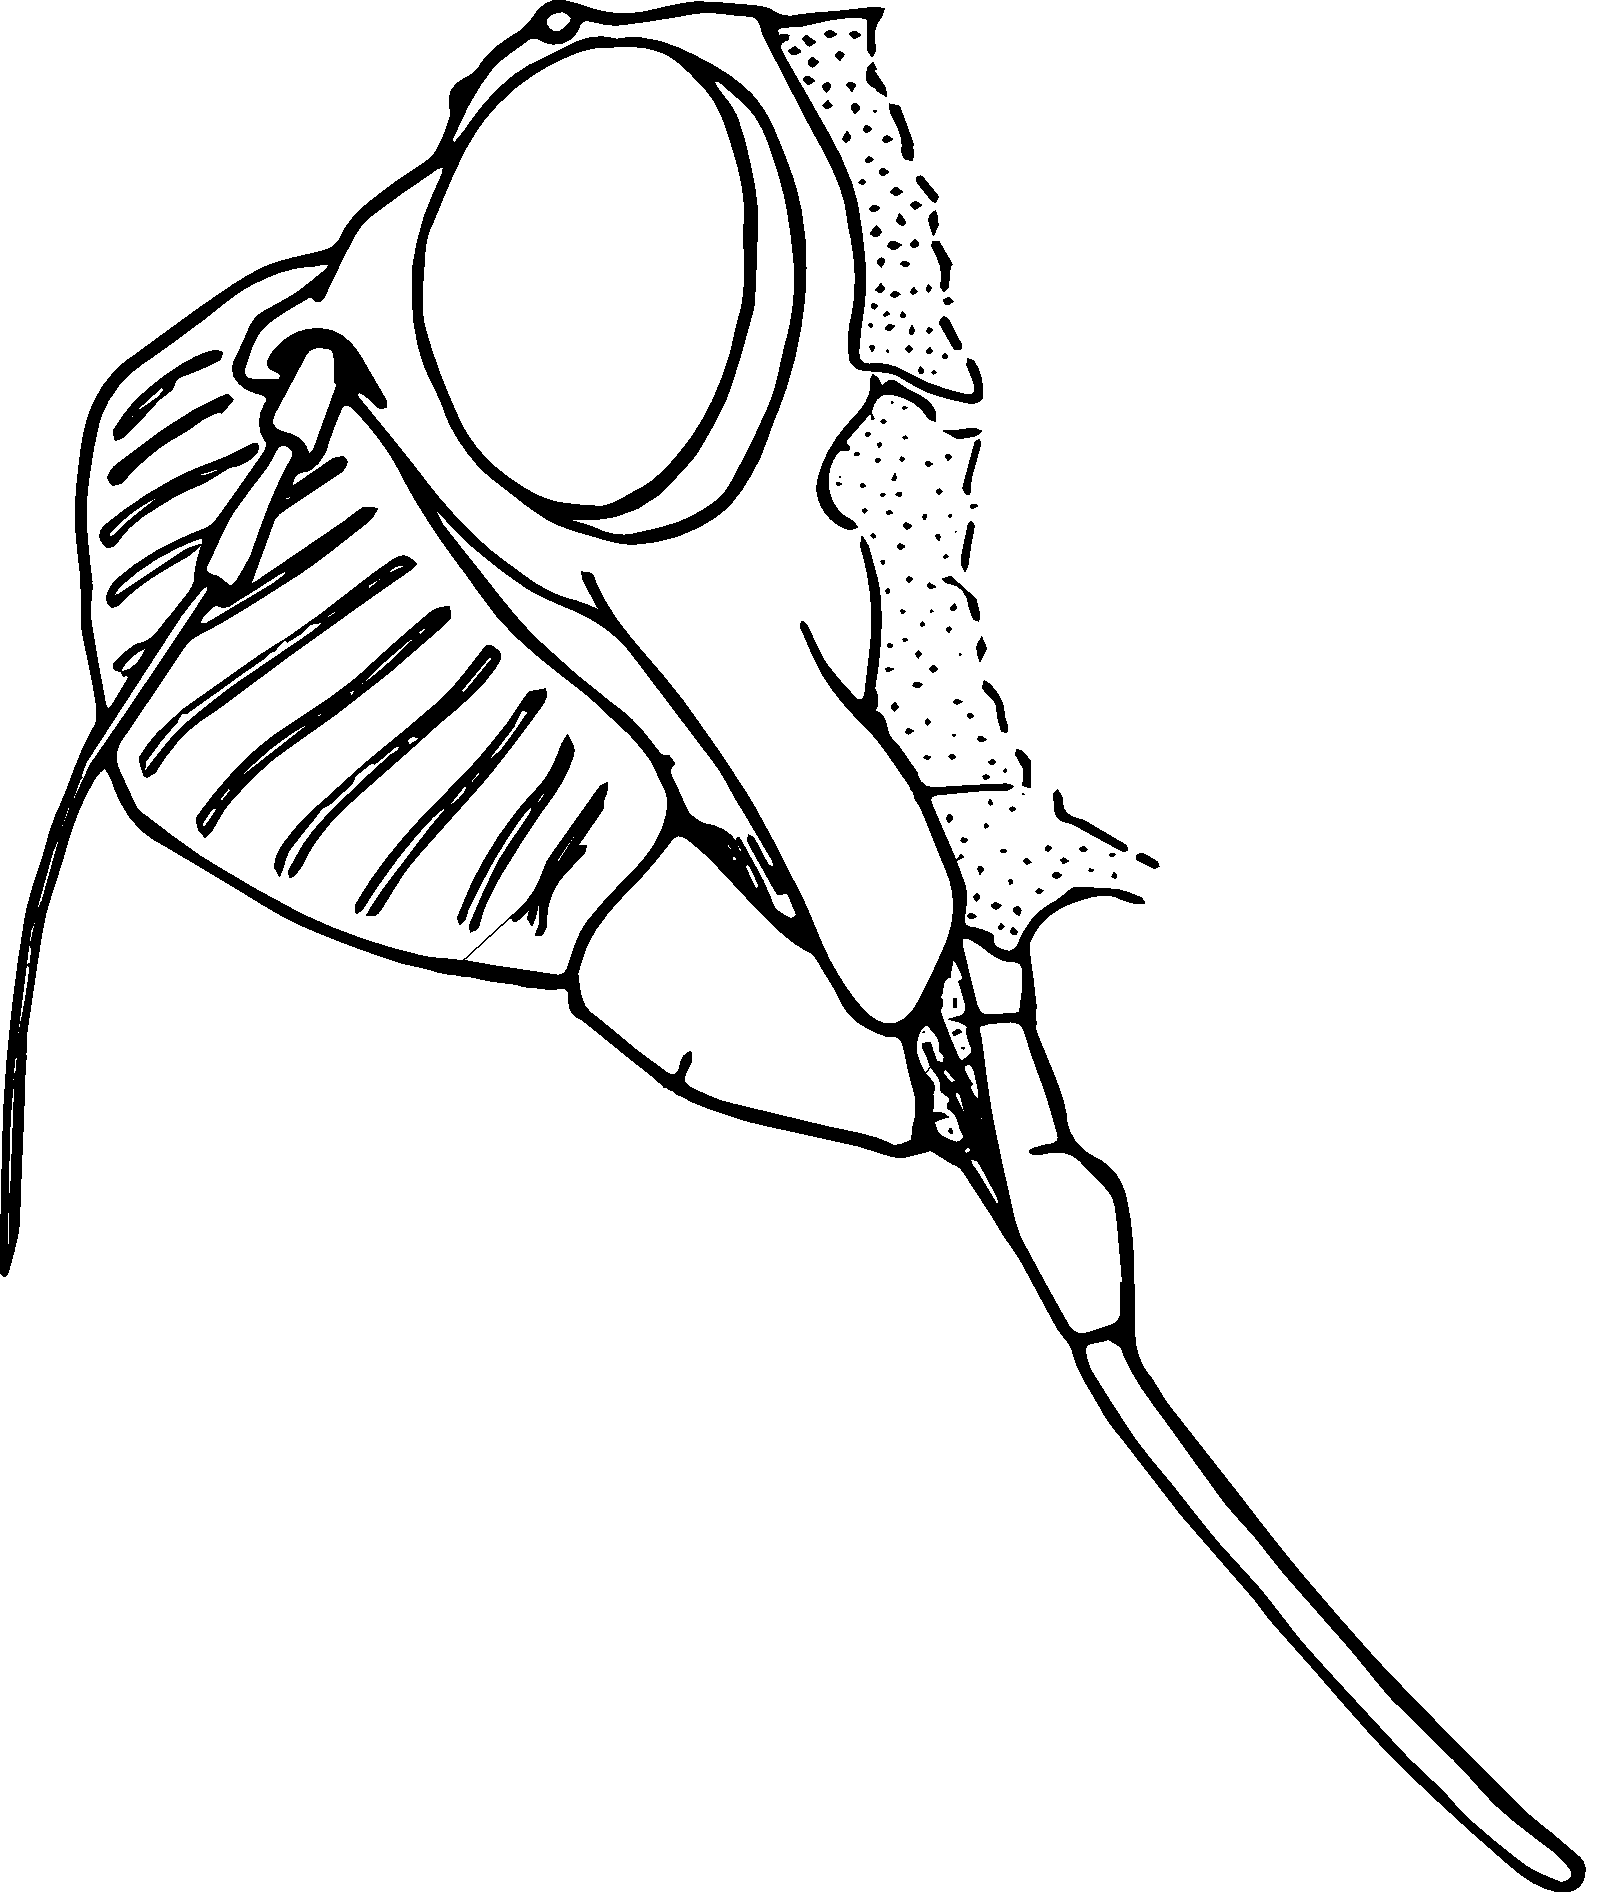
\includegraphics[width=\textwidth]{morphology/headCicada}
        \caption{}
        \label{fig:cicadaHead}
    \end{subfigure}
    \qquad
    \begin{subfigure}[ht!]{0.6\textwidth}
        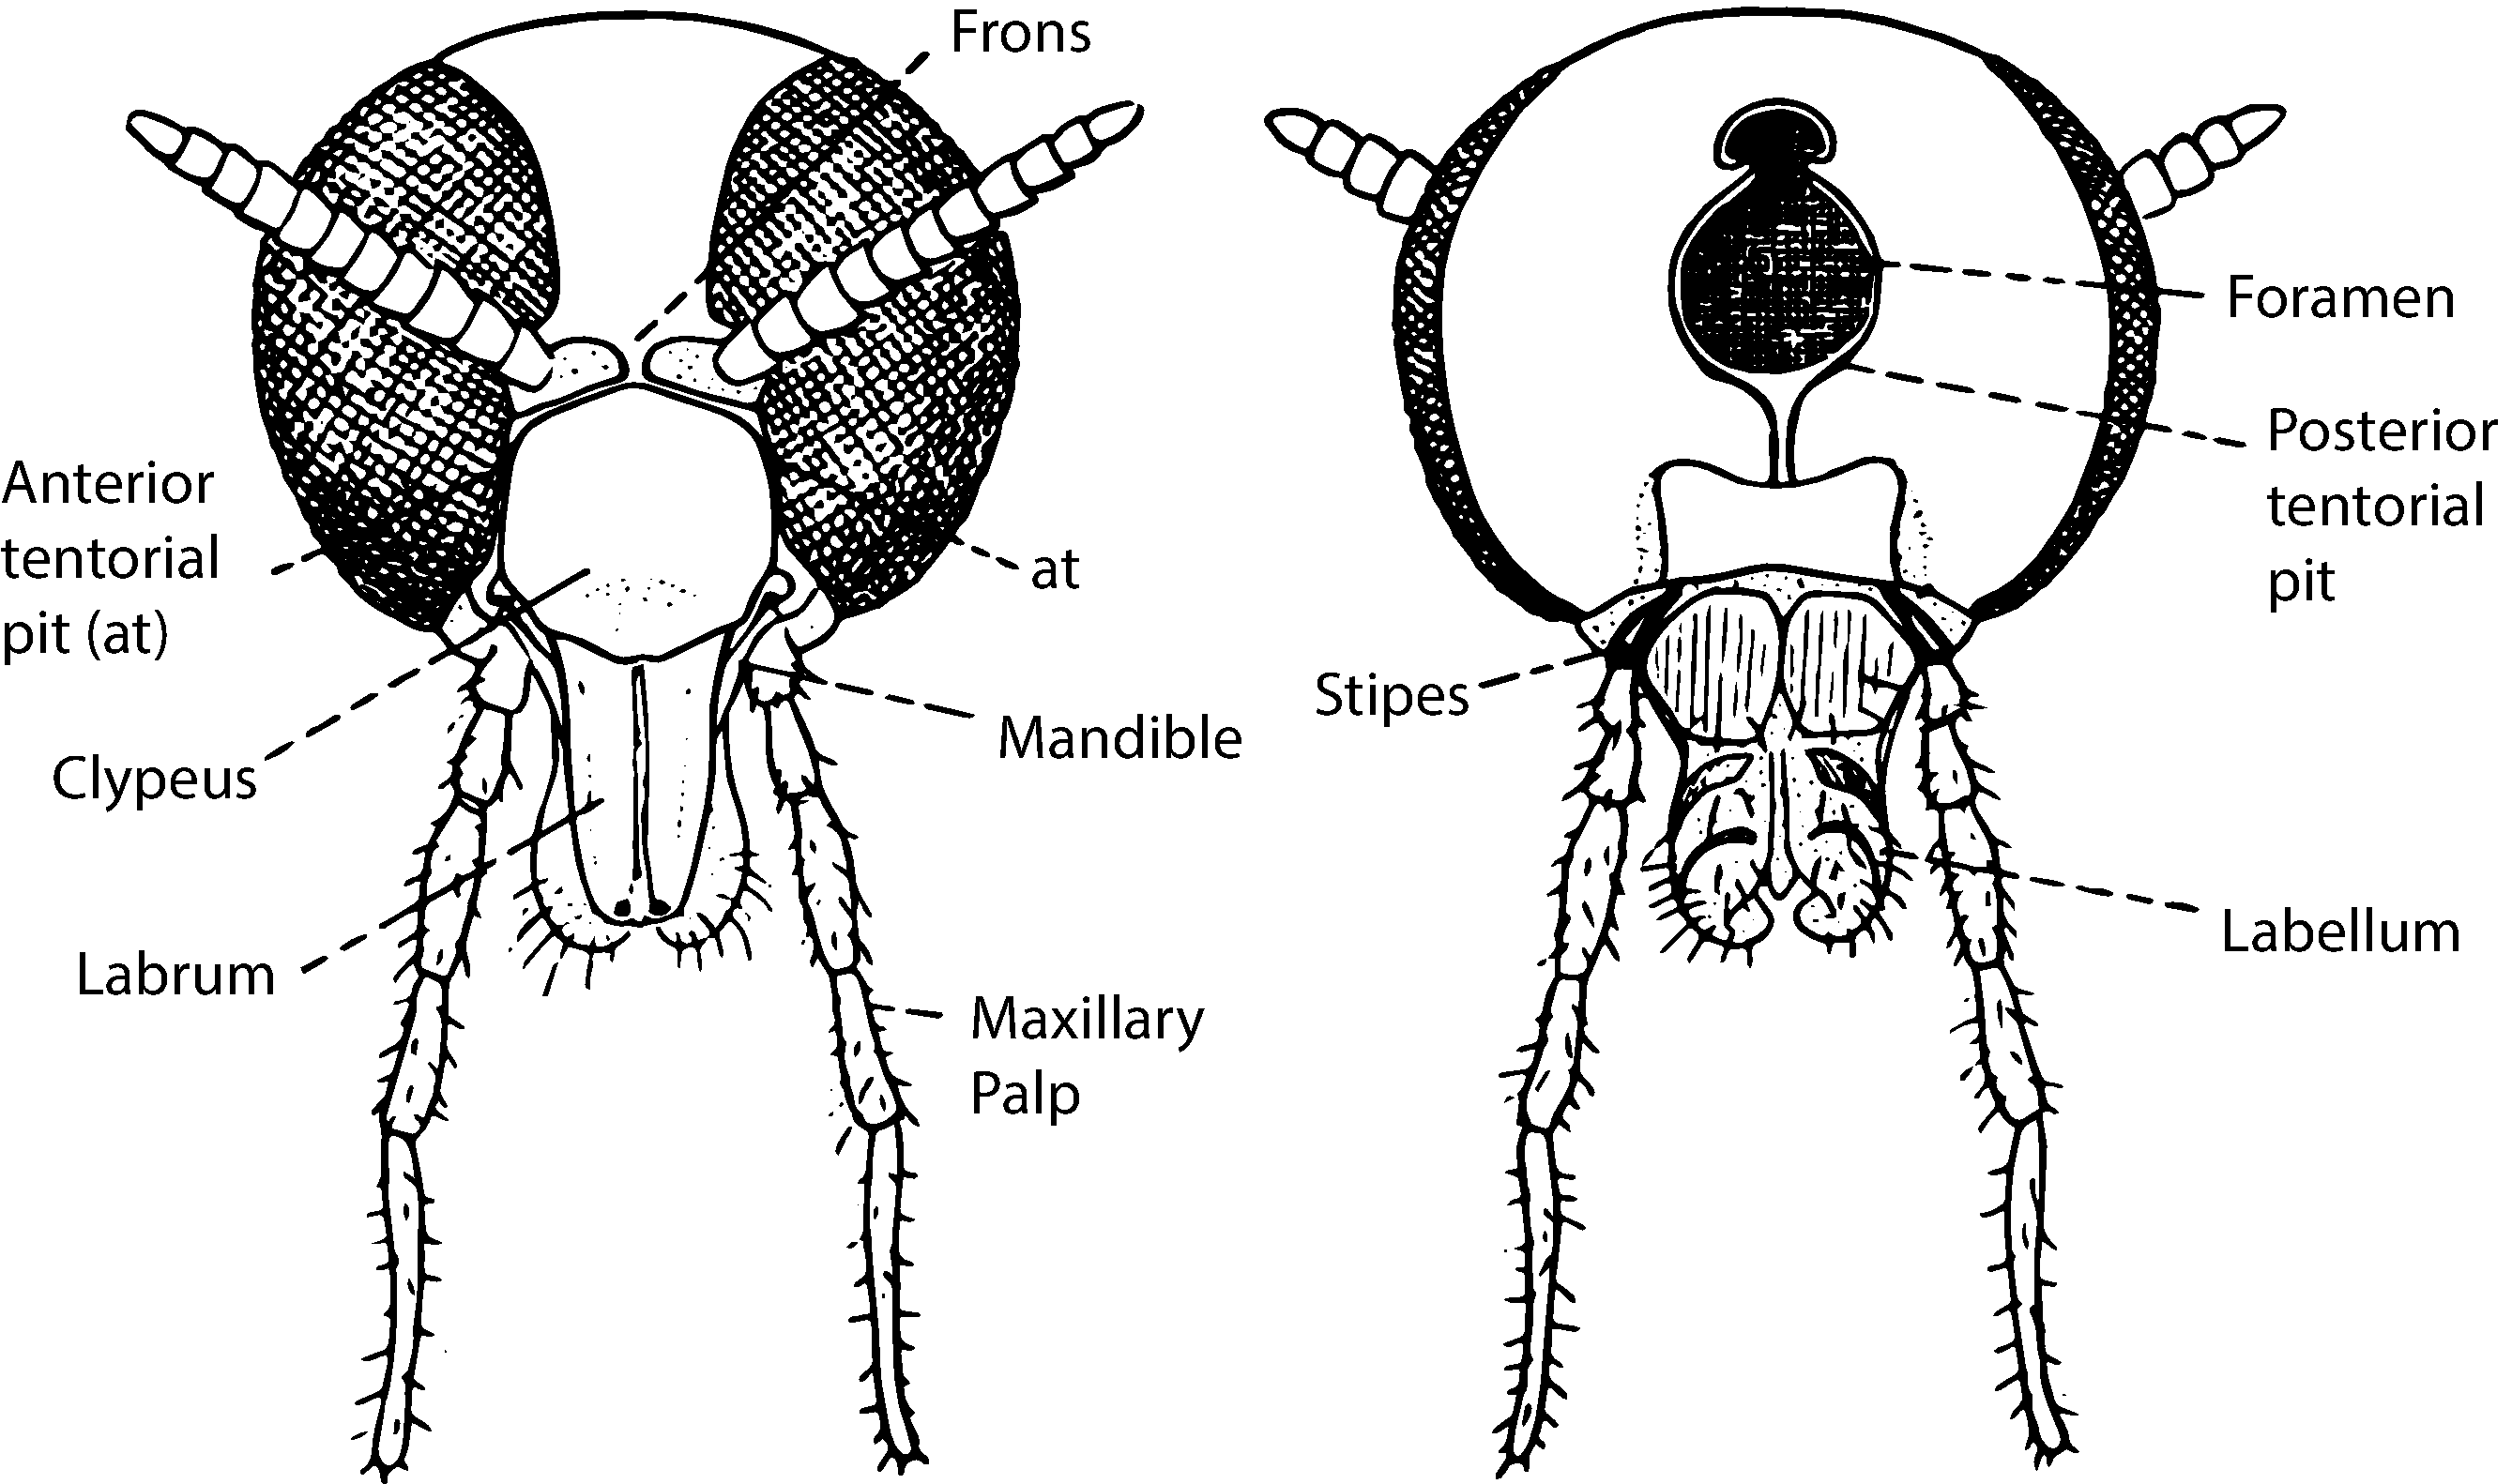
\includegraphics[width=\textwidth]{morphology/headFly}
        \caption{}
        \label{fig:headFly}
    \end{subfigure}
    \caption{Insect heads. \textbf{(a)} Cicada head \citep[redrawn from ][Fig. 121]{bhl128276}; \textbf{(b)} black fly head, anterior and posterior \citep[redrawn from][Fig. 24A,B]{snodgrass1944feeding}}
\end{figure}

\noindent{}Note the orientation of mouthparts in different specimens: projecting anteriorly\\ (\latinword{prognathous}), ventrally (\latinword{hypognathous}), or posteriorly (\latinword{opisthognathous}). These different orientations reflect modifications of the \latinword{cranium}. Find an example of each in your set of specimens.\vspace{3mm}

\noindent{}Once you're comfortable with insect mouthparts, see if you can understand the mouthparts of your arachnids.\vspace{3mm}

\begin{theo}[traits5]
{}What might be the function of the labrum, maxilla, and labium? Are these structures (plus the mandibles) present on all your specimens?\vspace{3mm}

\noindent{}Select the five arthropods you think have the greatest variation in mouthpart morphology: a fly, a bug, a spider, \textit{etc}. Describe and explain your hypotheses about the primary foods for each of these specimens? \vspace{3mm}

\noindent{}What might be the reason or function of these different mouthpart positions? How do these reflect their life history and habitats?
\end{theo}

\begin{figure}[ht!]
  \centering
    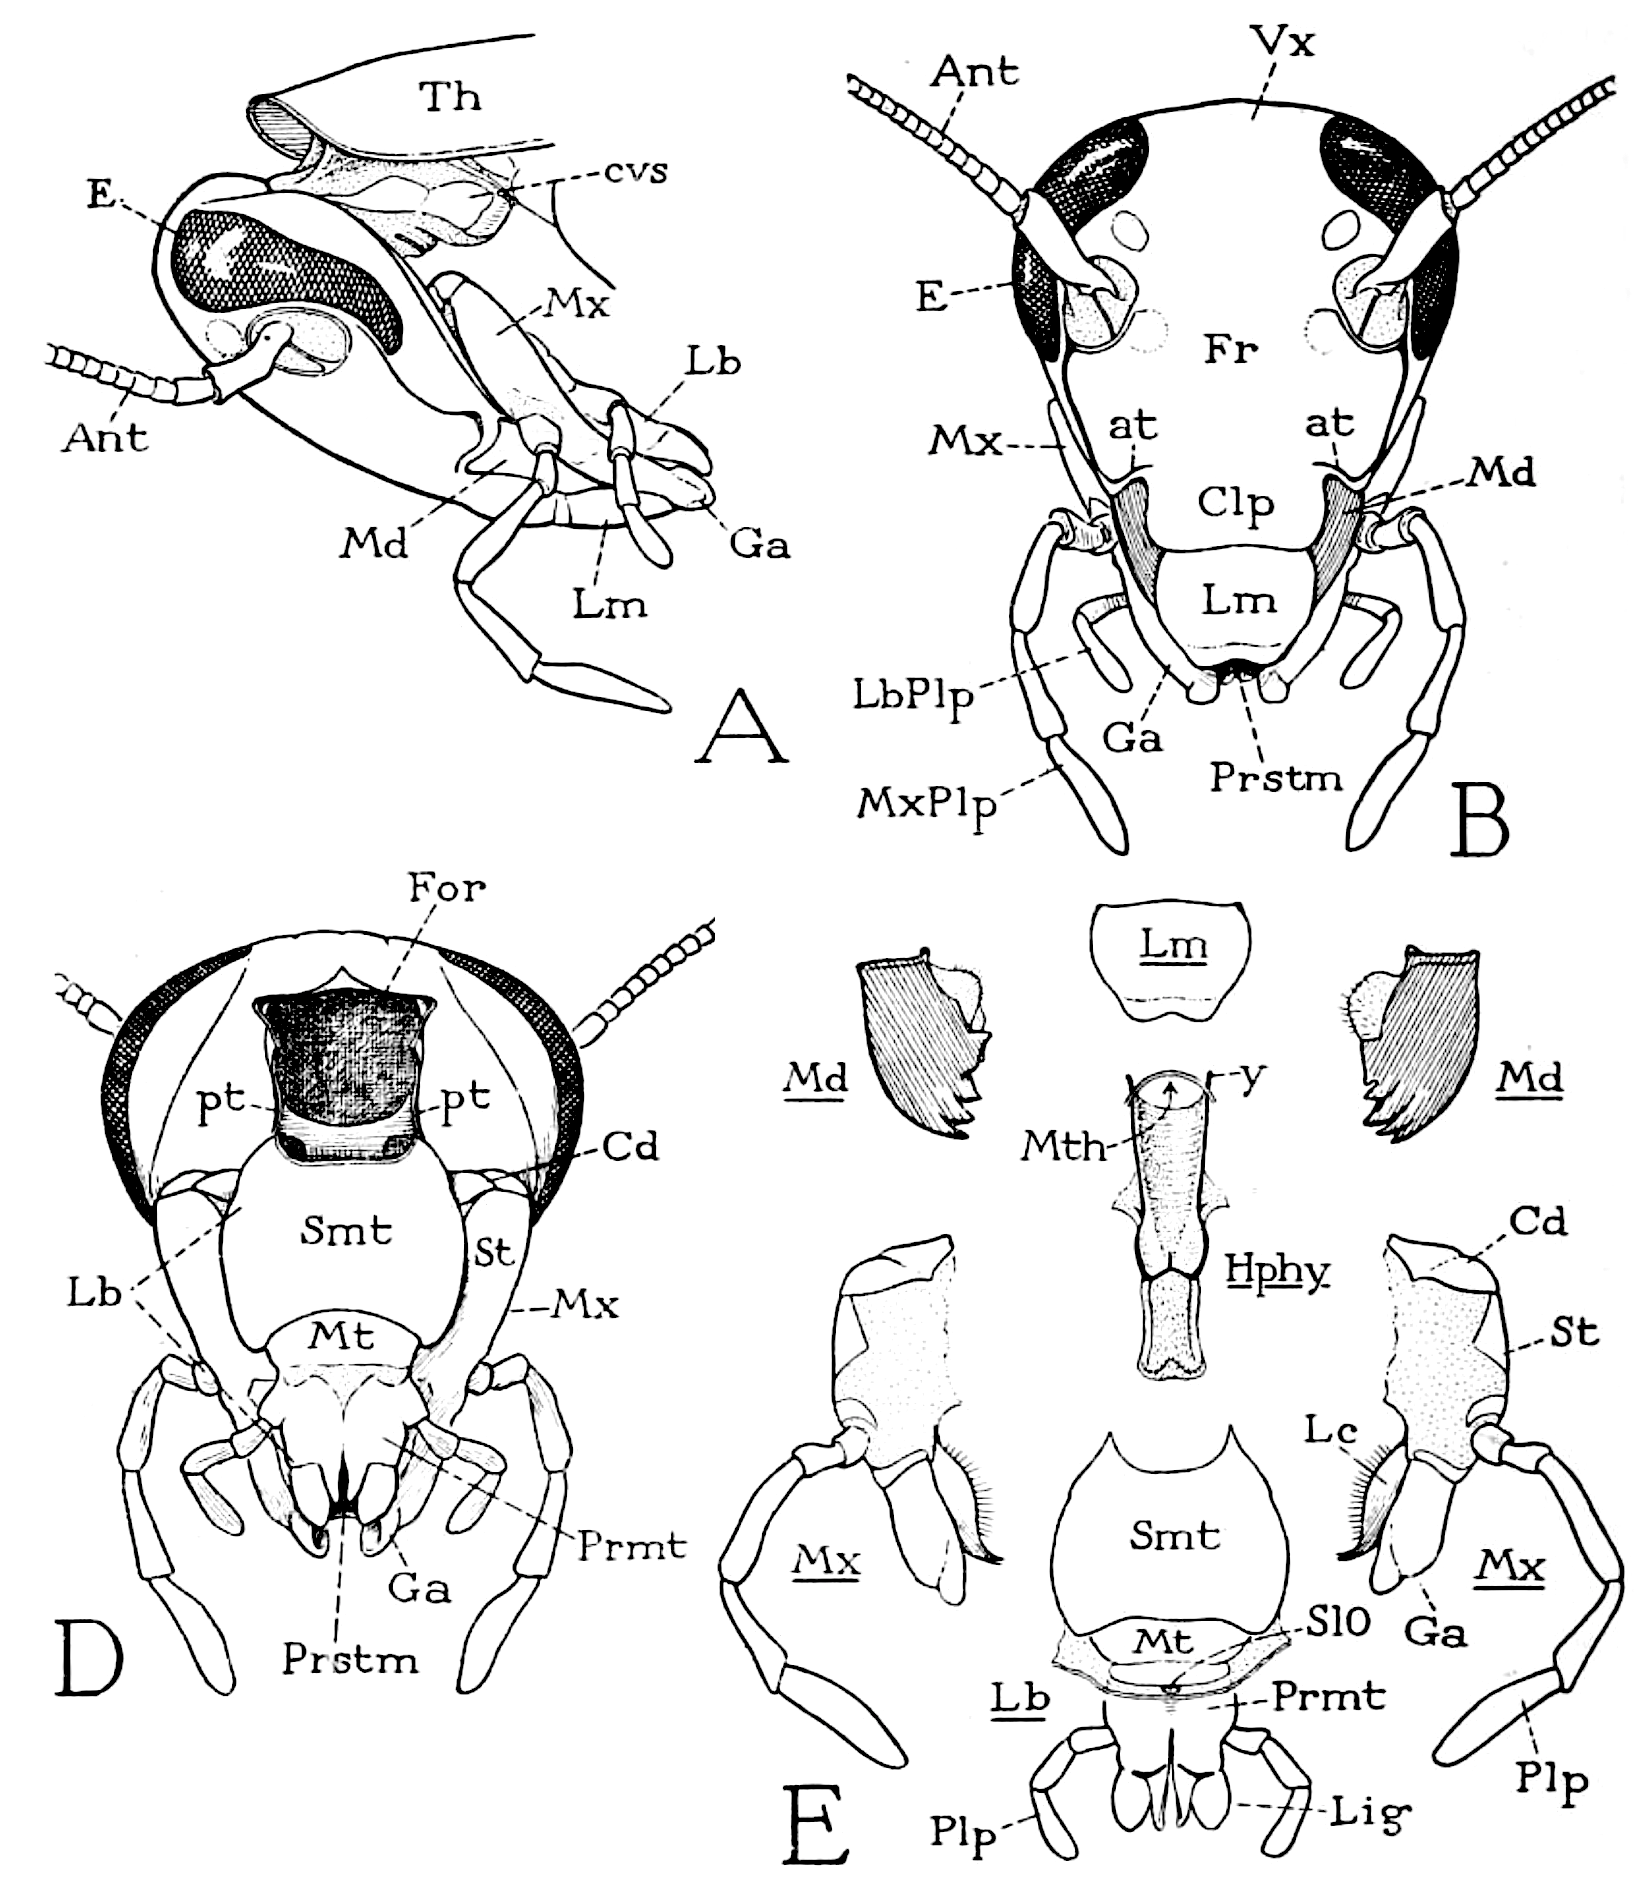
\includegraphics[width=0.7\textwidth]{morphology/headCockroach}
  \caption{Cockroach head. \citep[][Fig. 2A--E]{snodgrass1944feeding}}
  \label{fig:headCockroach}
\end{figure}

\noindent{}Eyes are used for vision and light detection. Locate them on your specimens and think about how they are differentiated from the rest of the body (cuticle). Compare the eyes of the insect specimens to those of non-insects.\vspace{3mm}

\begin{theo}[traits6]
{}What might be the function of a \latinword{compound eye} \textit{vs}. an \latinword{ocellus} (\latinword{-i})? How might spider vision differ from insect vision?
\end{theo}

\section{Thorax}
Posterior to the head is another tagma called the \latinword{thorax}. As with the head, examine each specimen for evidence of segmentation. See if each specimen even has a thorax. Compare a spider to an insect, for example. Try to determine how many segments comprise this tagma---you'll probably see three, the \latinword{prothorax}, \latinword{mesothorax}, and \latinword{metathorax}---and think about the tagma's primary function.\vspace{3mm}

\begin{theo}
{}In extant insects, the first thoracic segment does not bear a wing. Why? Does this body region serve other functions?
\end{theo}\vspace{3mm}

\noindent{}In your hexapod specimens, find sclerites you think represent the \latinword{notum}, \latinword{sternum}, and \latinword{pleuron}. Note that the surfaces of the nota of many insects have \latinword{furrows}, separating convex regions.\vspace{3mm}

\begin{figure}[ht!]
  \centering
    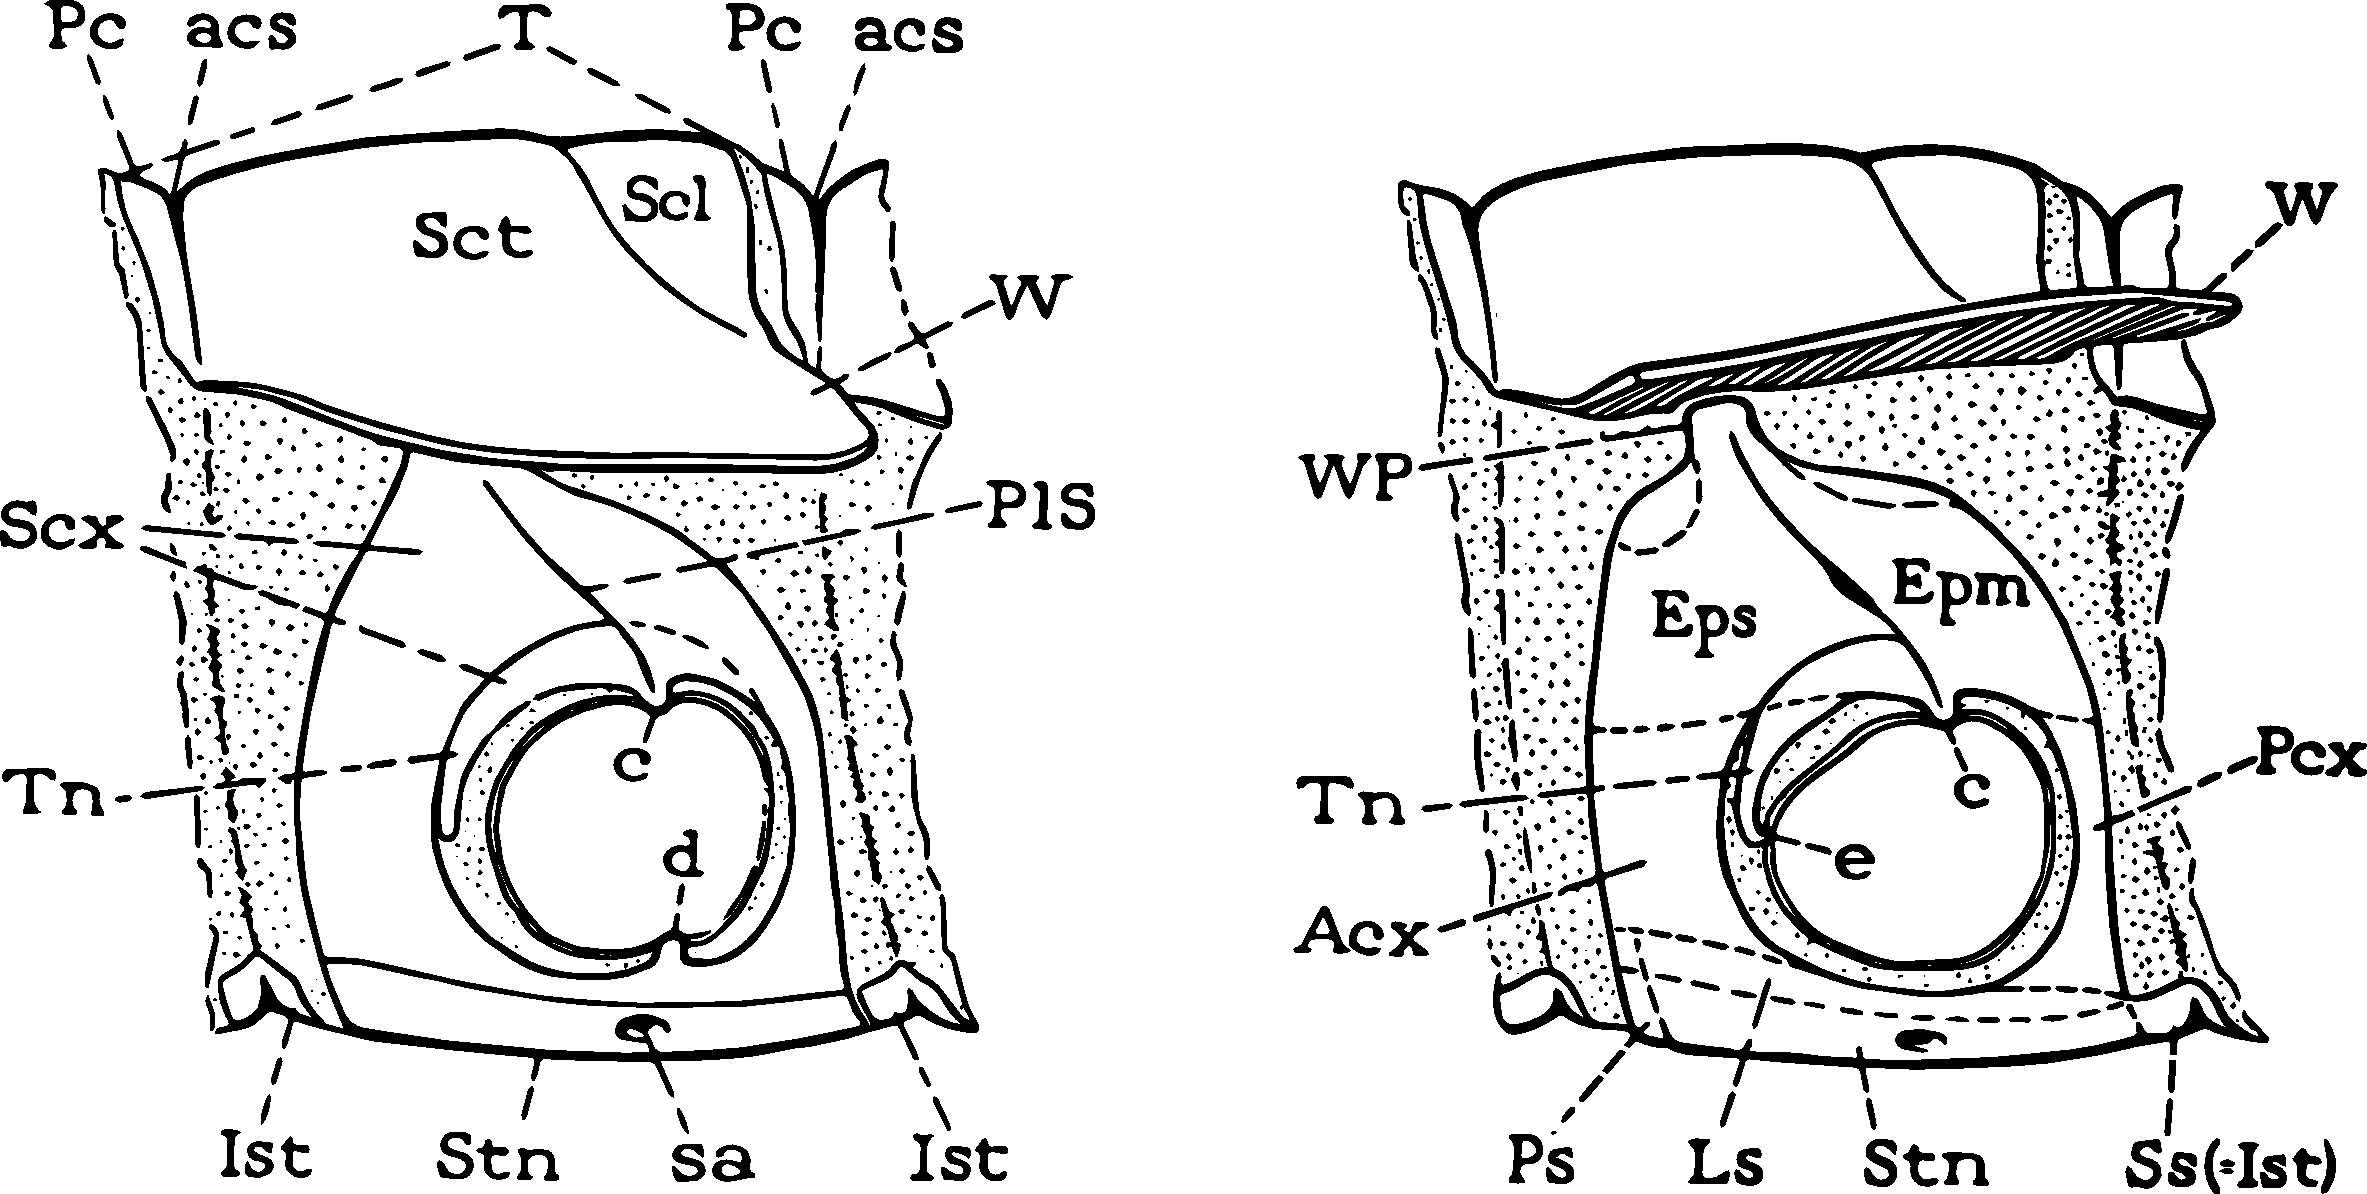
\includegraphics[width=0.8\textwidth]{morphology/scleritesThorax}
  \caption{Generalized thoracic segments, prothorax (left) and mesothorax (right). Antecostal suture (acs); dorsal (c) and ventral (d) subcoxo-coxal articulations; epimeron (Epm) episternum (Eps); eupleuron (Eupl); eutrochantin (Eutn); primary intersegmental line (Isg); intersegmental intersternites (Ist); precosta (Pc); scutum (Sct); scutellum (Scl); sternal plate (Stn); subcoxa (Scx); tergum (T); trochantin (Tn); wing process (WP). \citep[][Fig. 13]{snodgrass1929thoracic}}
  \label{fig:sclerites}
\end{figure}

\begin{theo}
{}Arthropods don't have ``bones''; where do muscles attach, to facilitate movement? Can you find evidence of your hypothesis by looking externally at the arthropod?
\end{theo}\vspace{3mm}

\subsection{Legs}

\noindent{}Locate the following leg segments in your insects: \latinword{coxa}, \latinword{trochanter}, \latinword{femur}, \latinword{tibia}, \latinword{tarsus}, \latinword{tarsomere}, \latinword{pretarsal claw}. Now try to locate these segments on the arachnid specimens. (Hint: try counting the leg segments, to see if they're the same between insects and arachnids). Spend some time observing different specializations of insect legs. We'll talk about adaptations related to locomotion and other behaviors. Some terms to define: \latinword{ambulatorial}, \latinword{cursorial}, \latinword{saltatorial}, \latinword{natatorial}, \latinword{fossorial}, \latinword{raptorial}, \latinword{chelate}. We'll also examine apices of various arthropod legs, to find structures (\latinword{attachment devices}) that help them cling to smooth surfaces, like a leaf or a window.\vspace{3mm}

\begin{figure}[ht!]
    \centering
    \begin{subfigure}[ht!]{0.5\textwidth}
        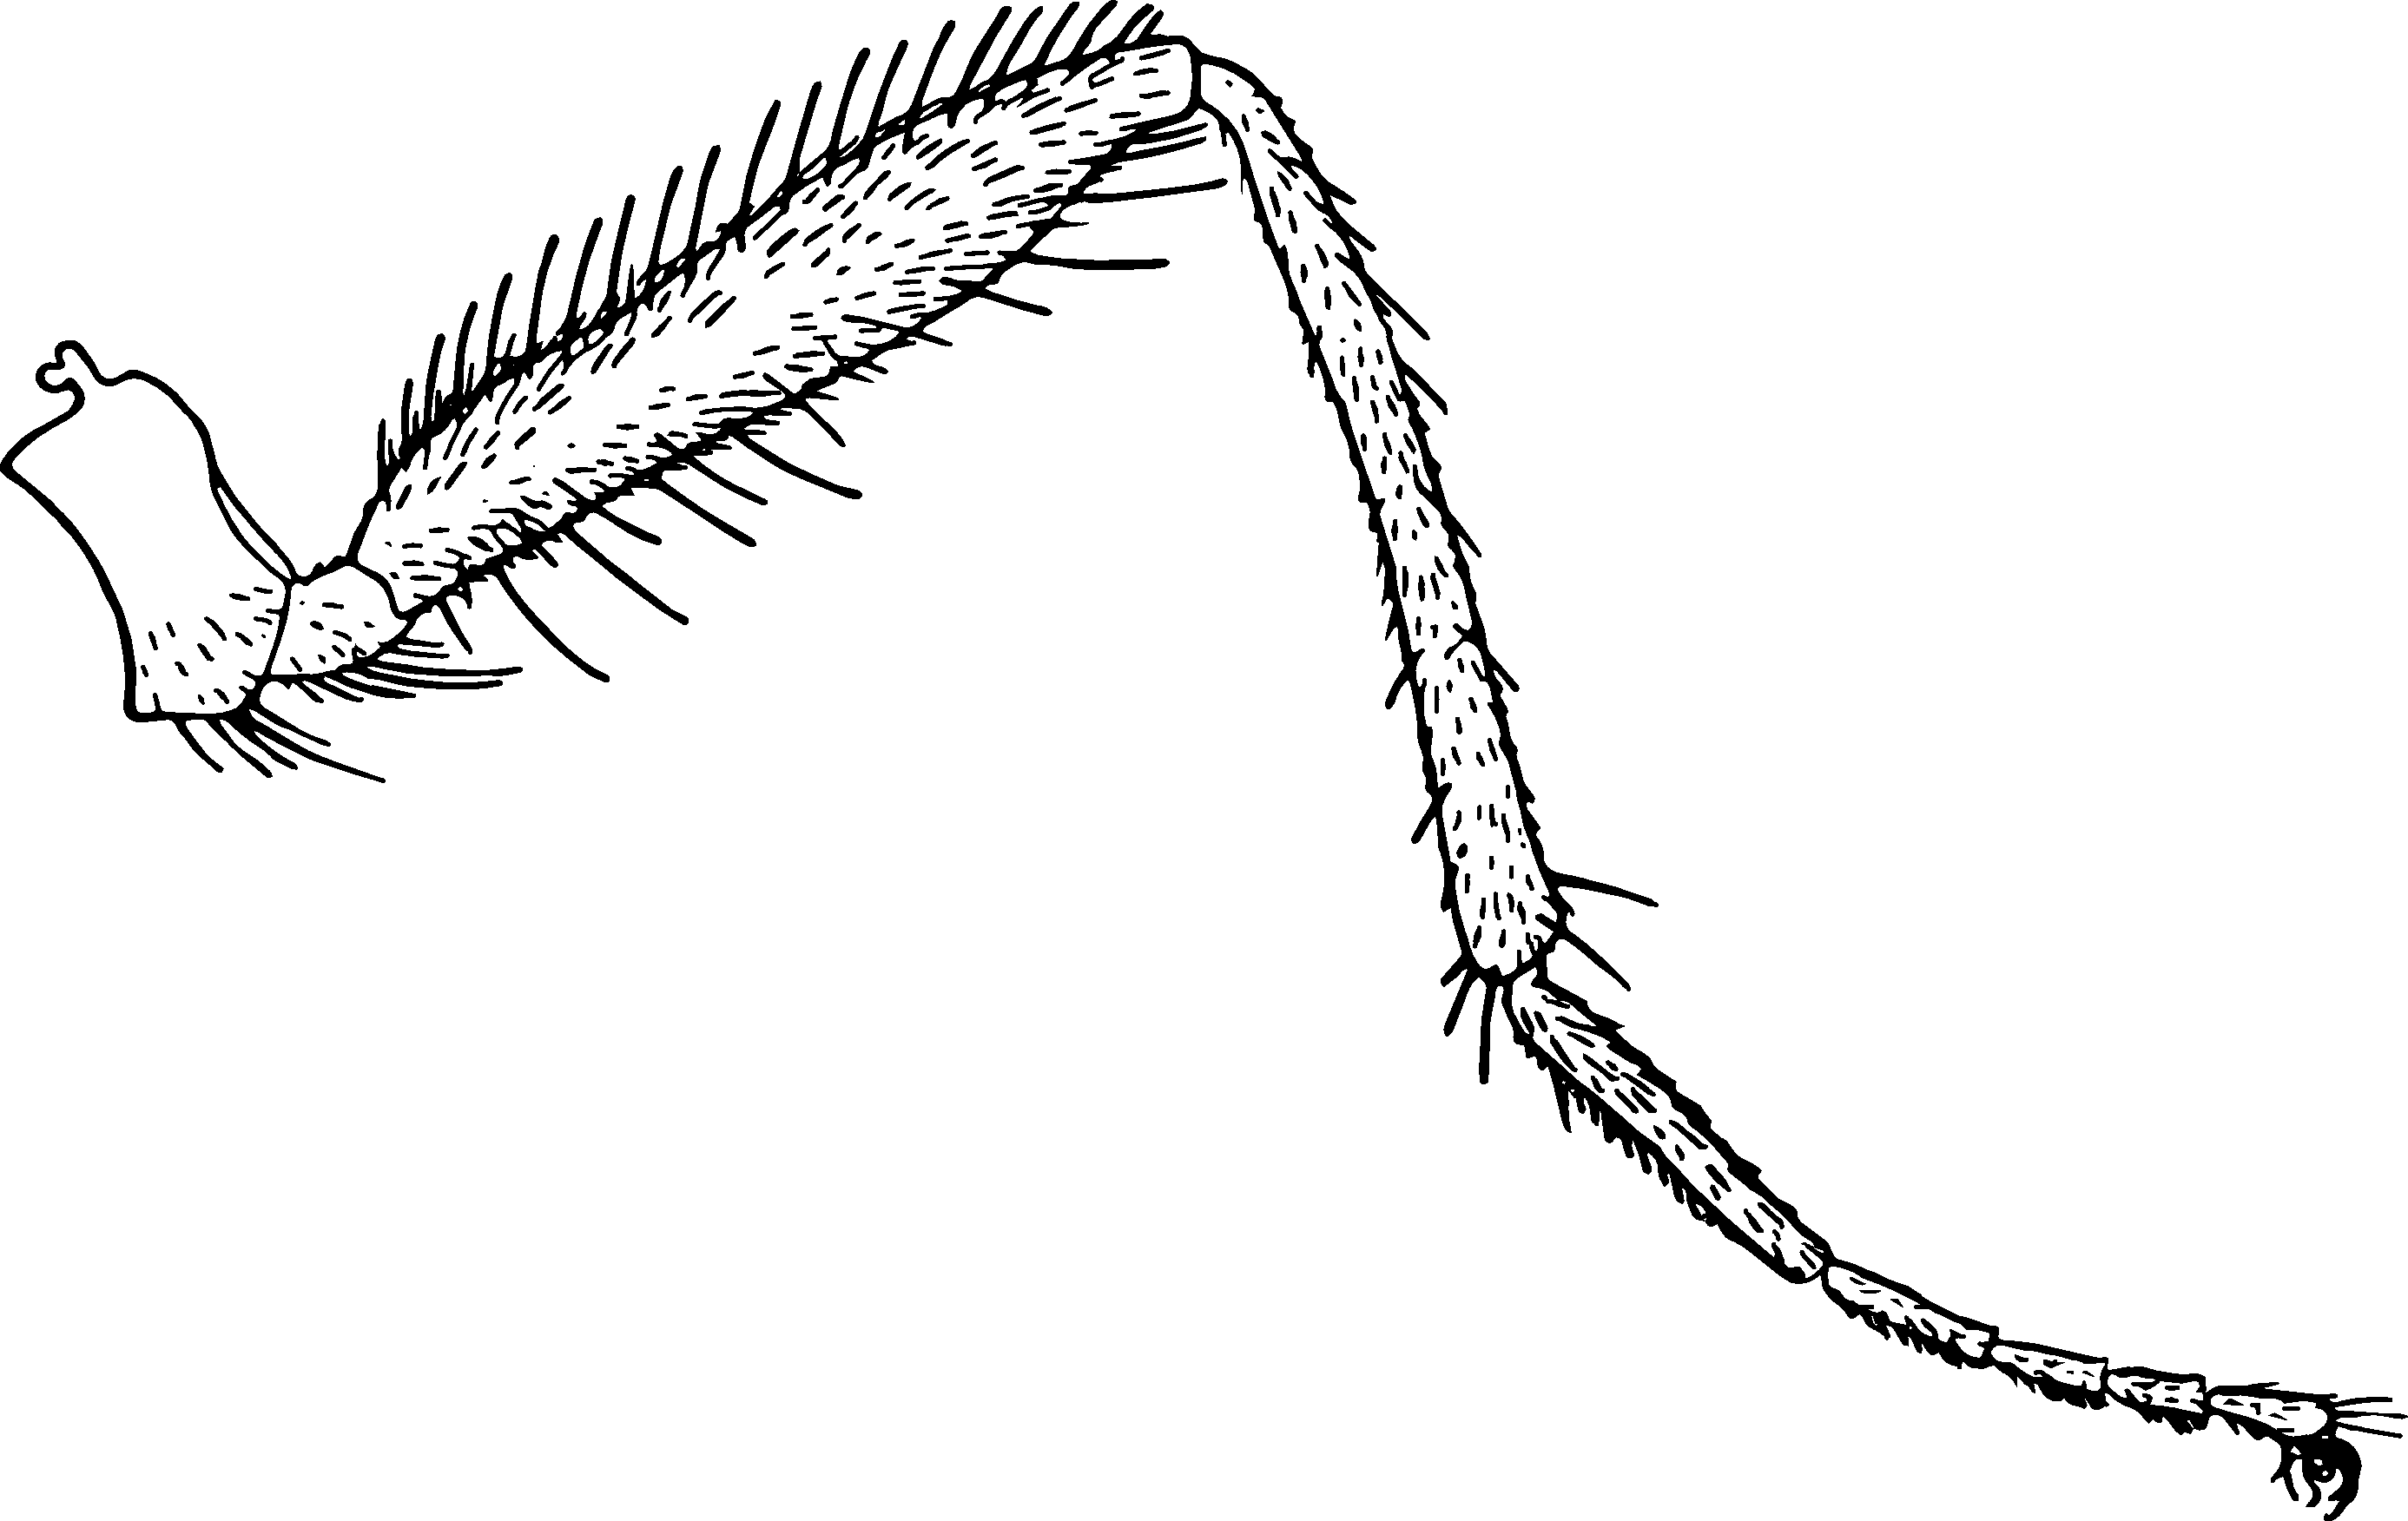
\includegraphics[width=\textwidth]{morphology/legSegments}
        \caption{}
        \label{fig:legSegments}
    \end{subfigure}
    \qquad
    \begin{subfigure}[ht!]{0.3\textwidth}
        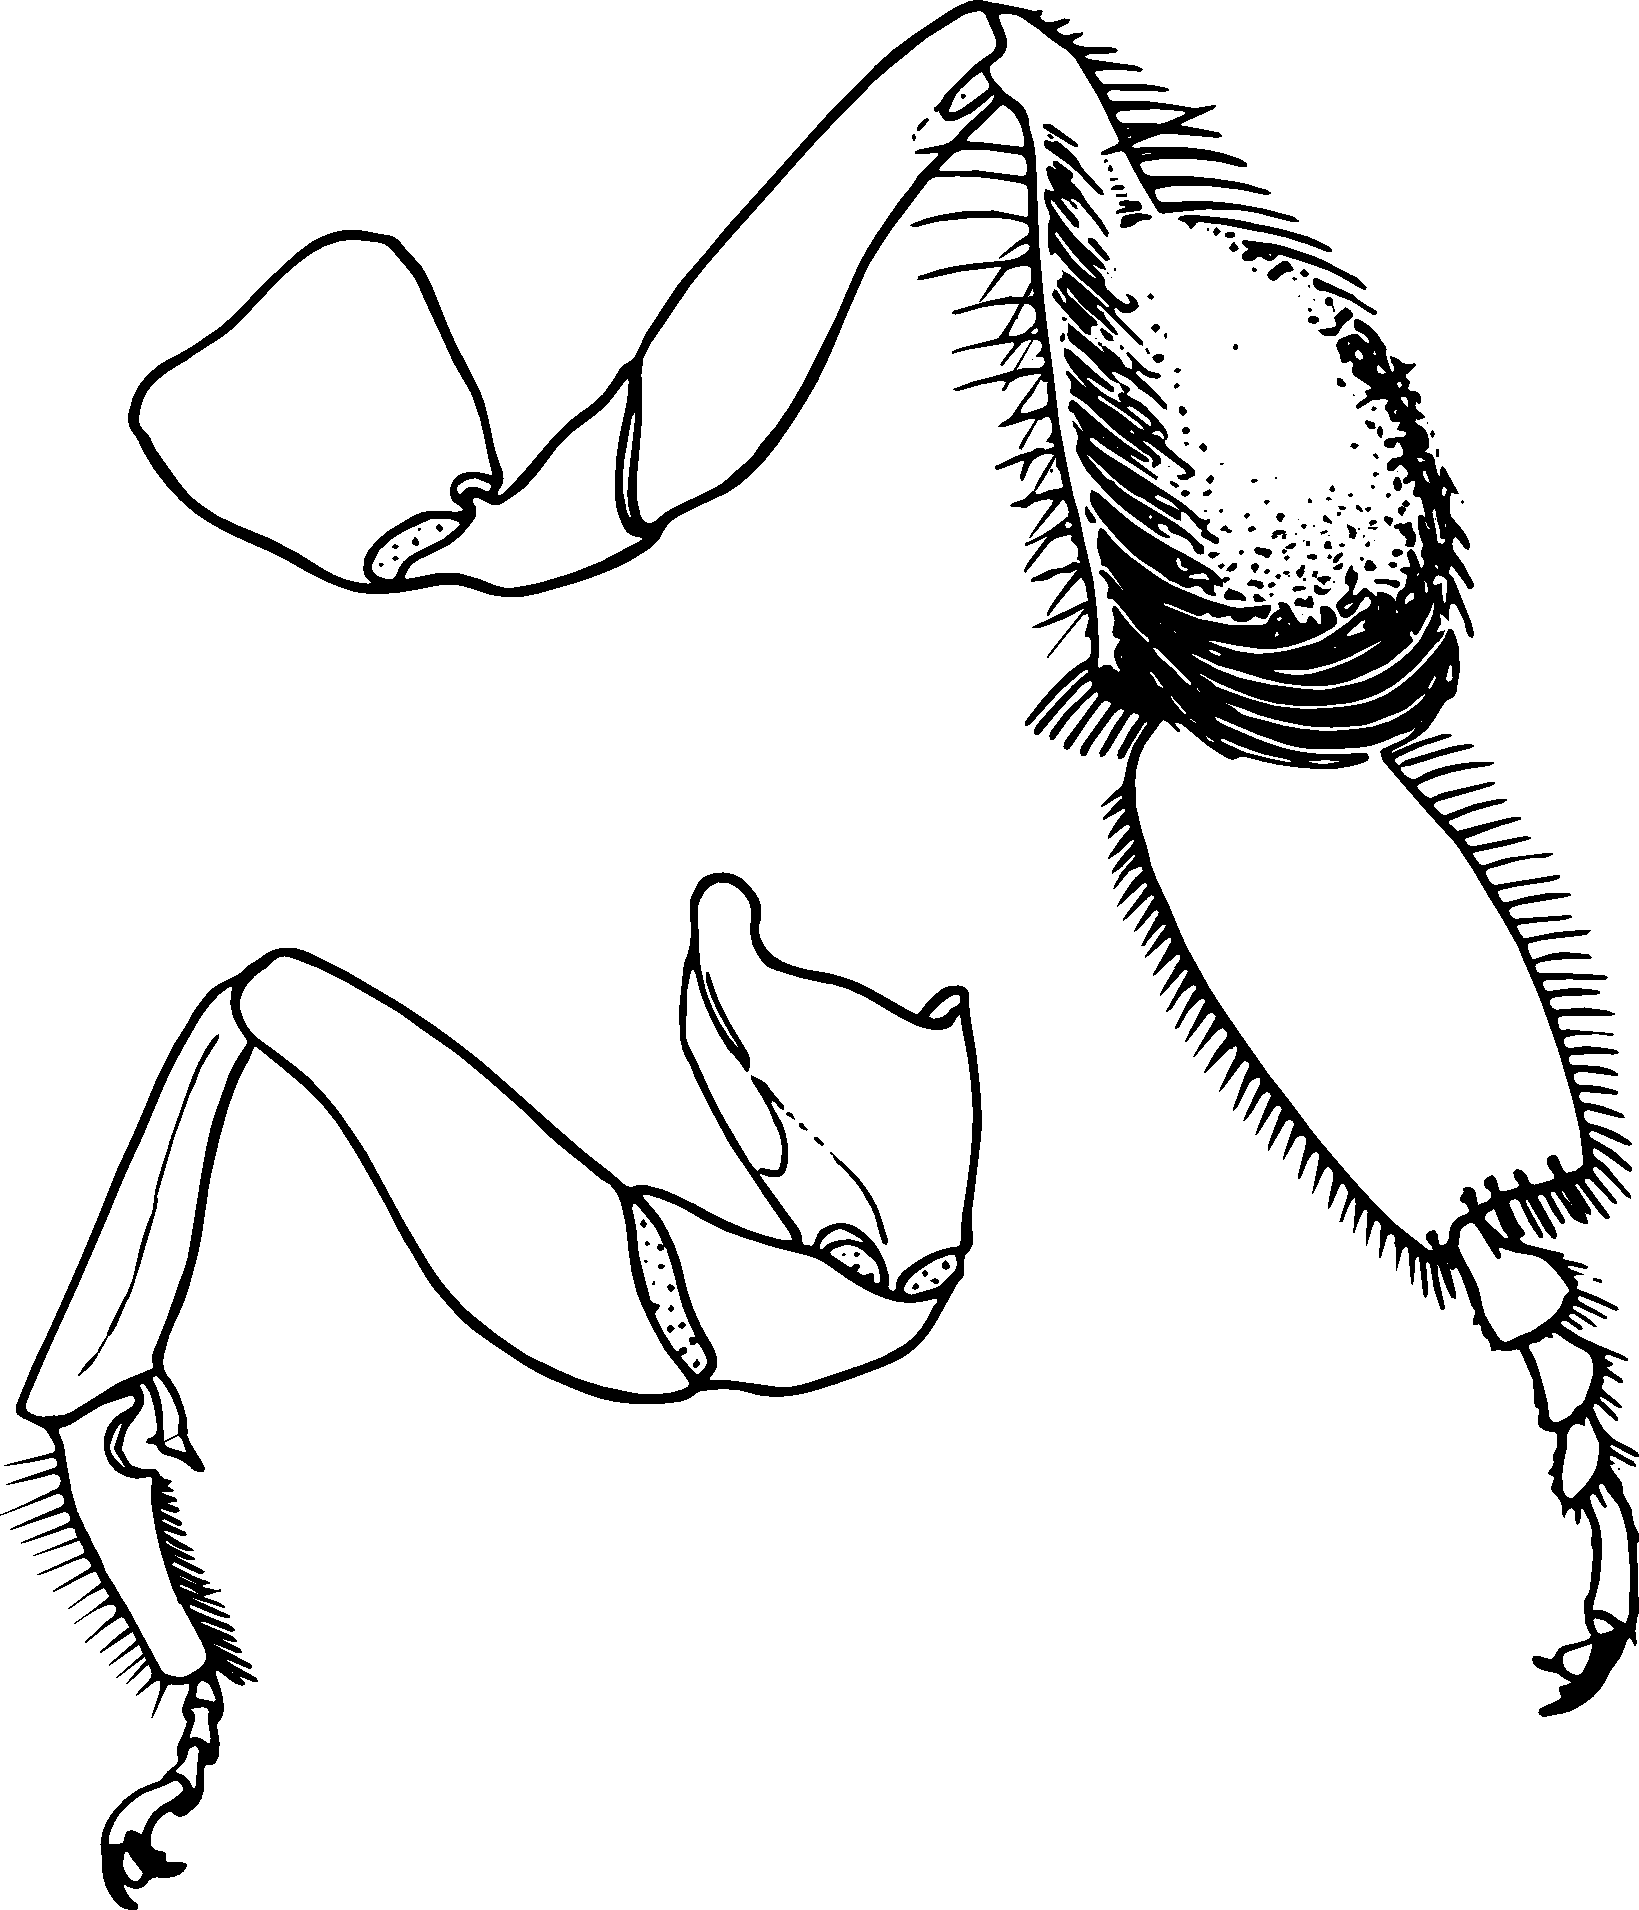
\includegraphics[width=\textwidth]{morphology/beeLegs}
        \caption{}
        \label{fig:beeLegs}
    \end{subfigure}
    \caption{Insect legs. \textbf{(a)} Aimple leg \citep[][Fig. 24, after Snodgrass]{bhlitem16791elementary}; \textbf{(b)} honey bee legs, hind (top) and fore leg (bottom) \citep[][Fig. 65]{bhl128276}}
\end{figure}%move the caption to here

\begin{theo}
{}Find at least 5 specimens with very different leg morphologies. Can you hypothesize something about the natural history of these specimens, based on their leg phenotypes?
\end{theo}\vspace{3mm}

\noindent{}Locate the \latinword{fore wing} and the \latinword{hind wing} on all your insect specimens. Then locate the following veins in different specimens: \latinword{costa} (C), \latinword{subcosta} (Sc), \latinword{radius} (R), \latinword{cubitus} (Cu), \latinword{medius} (M), \latinword{anal} (A). Look also for structures that aren't necessarily veins (fold lines, for example) but which otherwise aid in the function of the wing. Think about the characteristics and parts of the wings that allow them to function for flight.\vspace{3mm}

\begin{figure}[ht!]
  \centering
    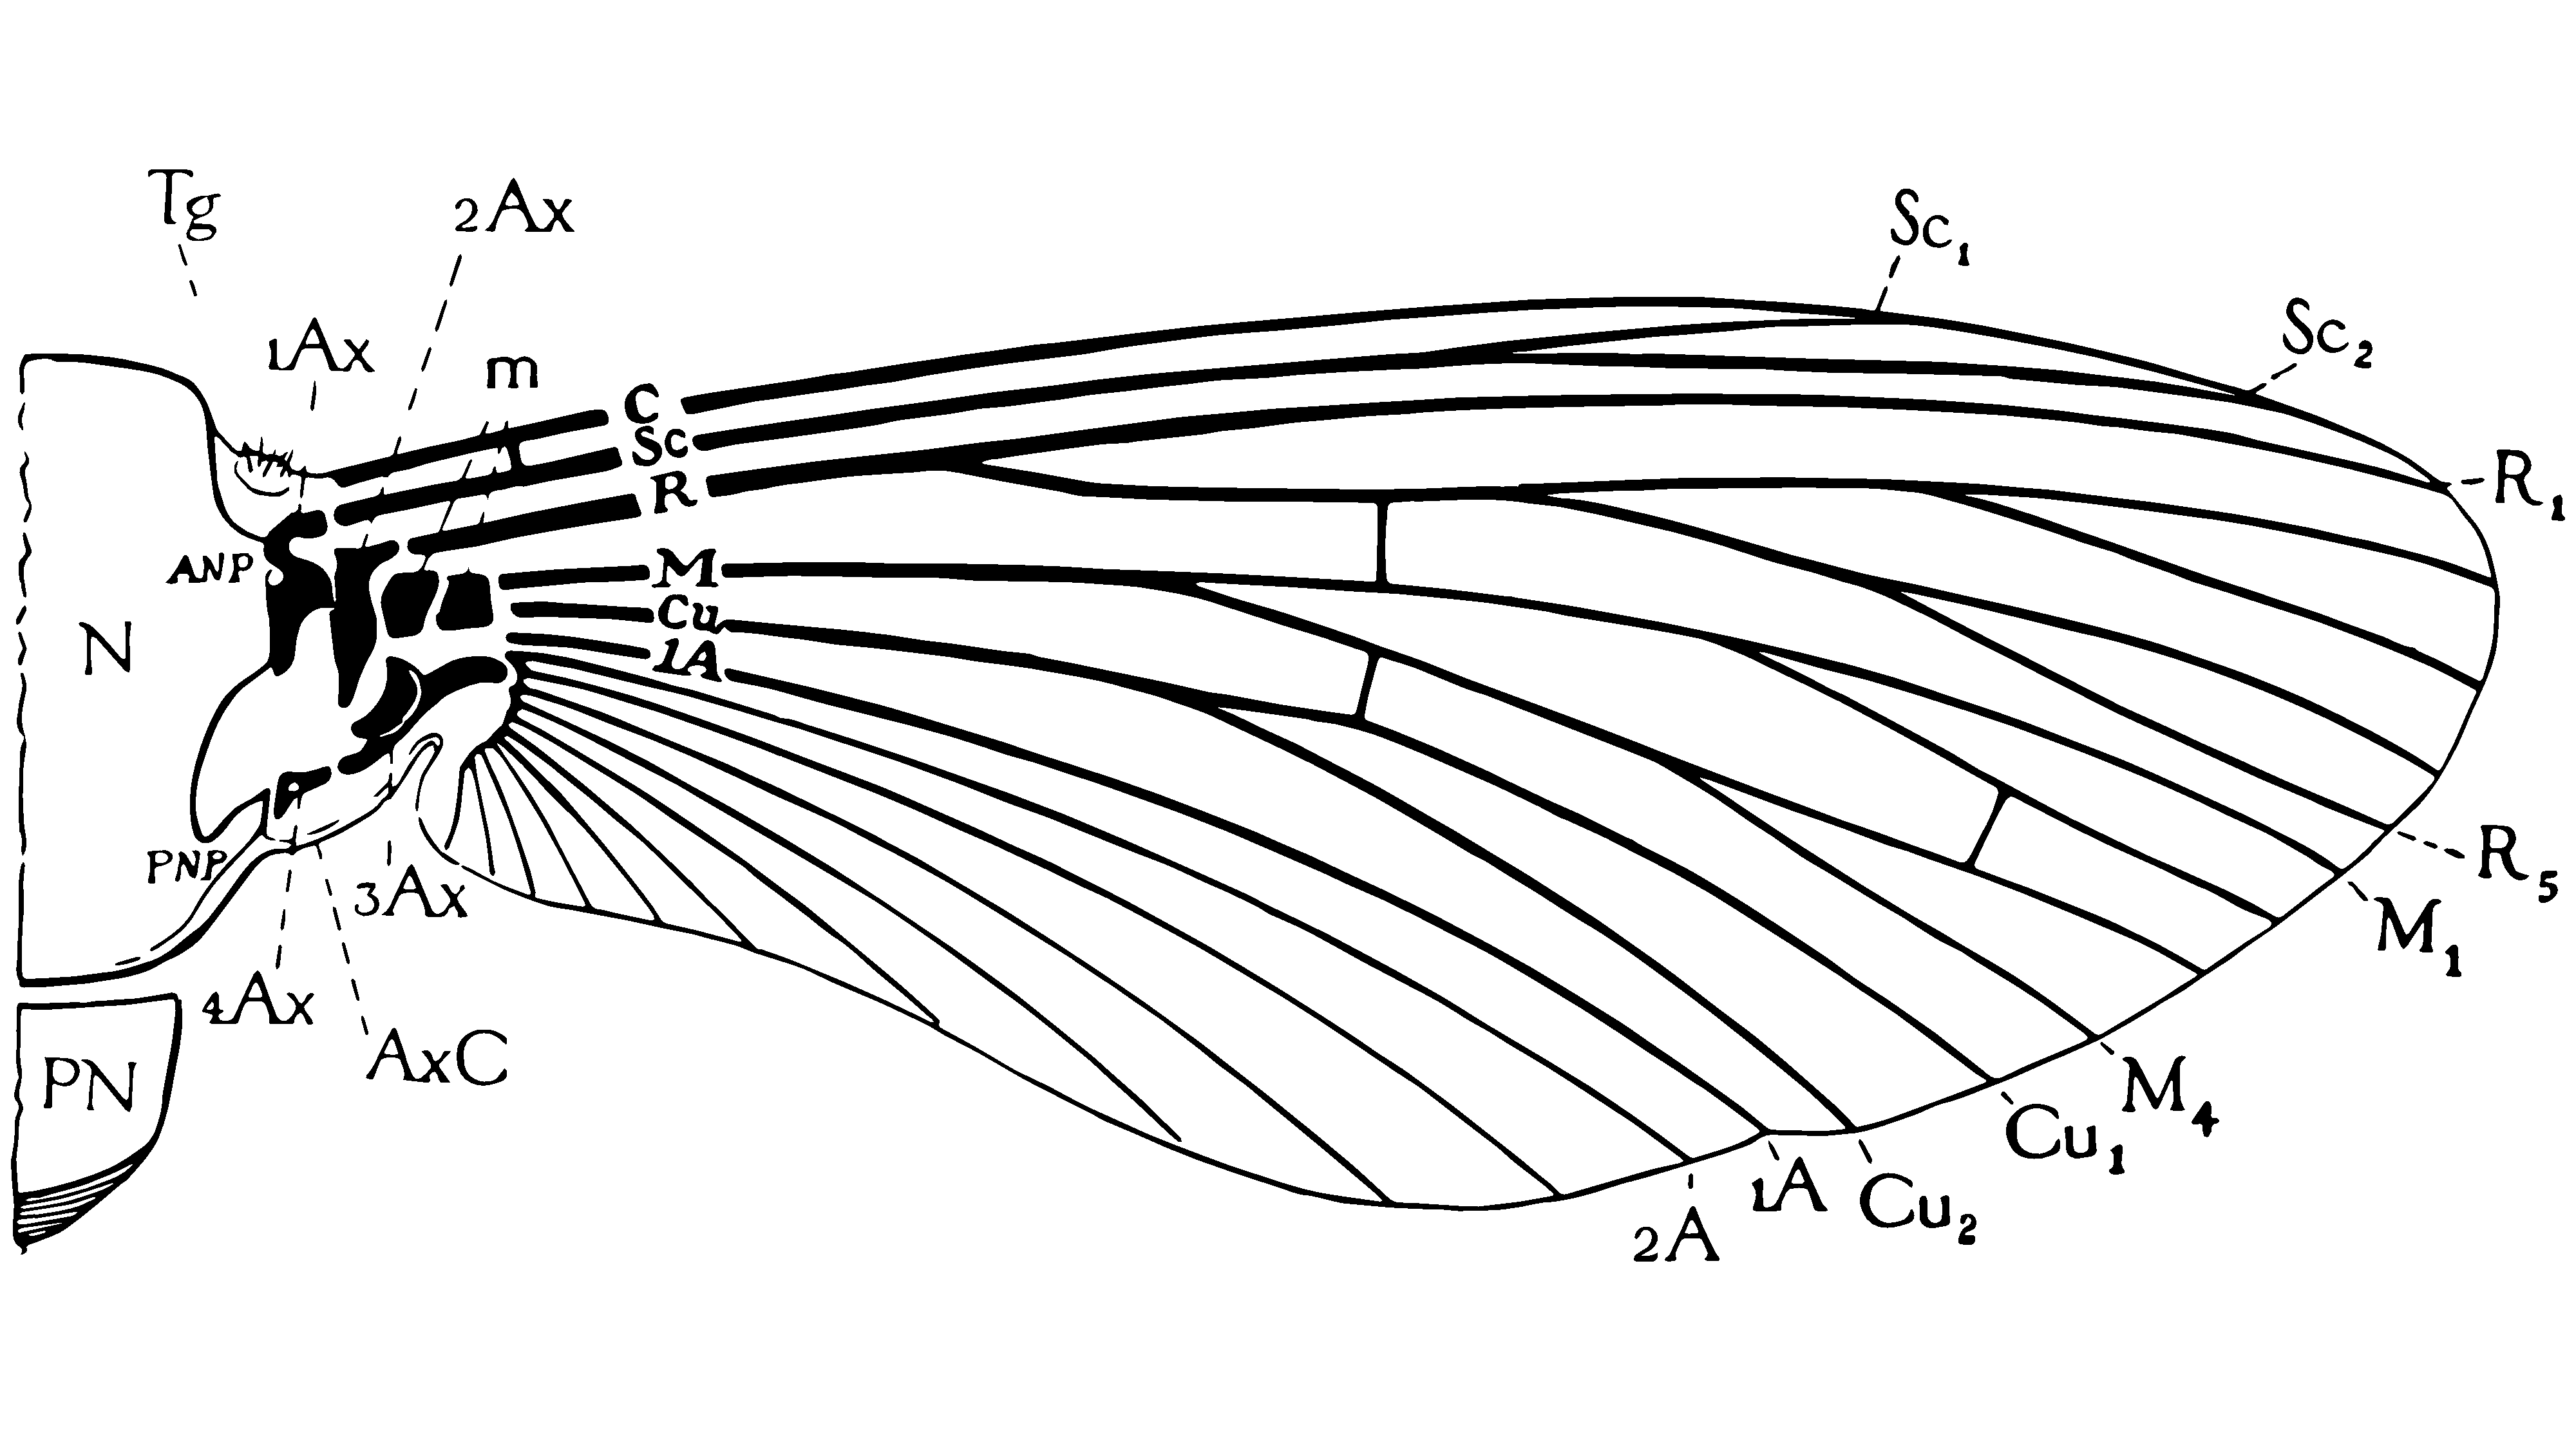
\includegraphics[width=0.8\textwidth]{morphology/wingveins}
  \caption{Generalized wing. \citep[][Fig. 6]{snodgrass1910honeybee}}
  \label{fig:wingveins}
\end{figure}

\begin{theo}
{}What might be the function of \latinword{wing veins}? Is it possible to homologize wing veins based on their orientation (relative to the anterior wing margin)? Do you see any patterns with respect to \latinword{crossveins} in your winged specimens?
\end{theo}\vspace{3mm}

\noindent{}Pay close attention to the wing morphology of beetles; we'll talk about the \latinword{elytron} (\latinword{-a}, plural). Given that the hind wing is so much larger than the elytron in your beetles, see if you can figure out how it fits under the fore wing.\vspace{3mm}

\noindent{}In some insects, Odonata for example, the fore and hind wings are used asynchronously during the flight. Hymenoptera, Lepidoptera, and some Heteroptera use the fore and hind wings simultaneously---\textit{i.e}., they function as a single wing. See if you can find anatomical structures that link or otherwise connect the two wings together.\vspace{3mm}

\section{Abdomen}
As with the tagmata above, see if you can find evidence for a third tagma posterior to the thorax---the \latinword{abdomen}---and for how many segments compose the structure.\vspace{3mm}

\noindent{}Look for appendages on the abdomen. Can you recognize male and female insects based on the tip of their abdomen? Think about the functions of the anatomical structures at the tip of the abdomen, for example the \latinword{cerci} (\latinword{cercus}, sing.) or the \latinword{ovipositor}.\vspace{3mm}

\begin{theo} 
{}The terminalia of the abdomen is key in species identification for numerous insect groups. Why?
\end{theo}

\begin{figure}[ht!]
  \centering
    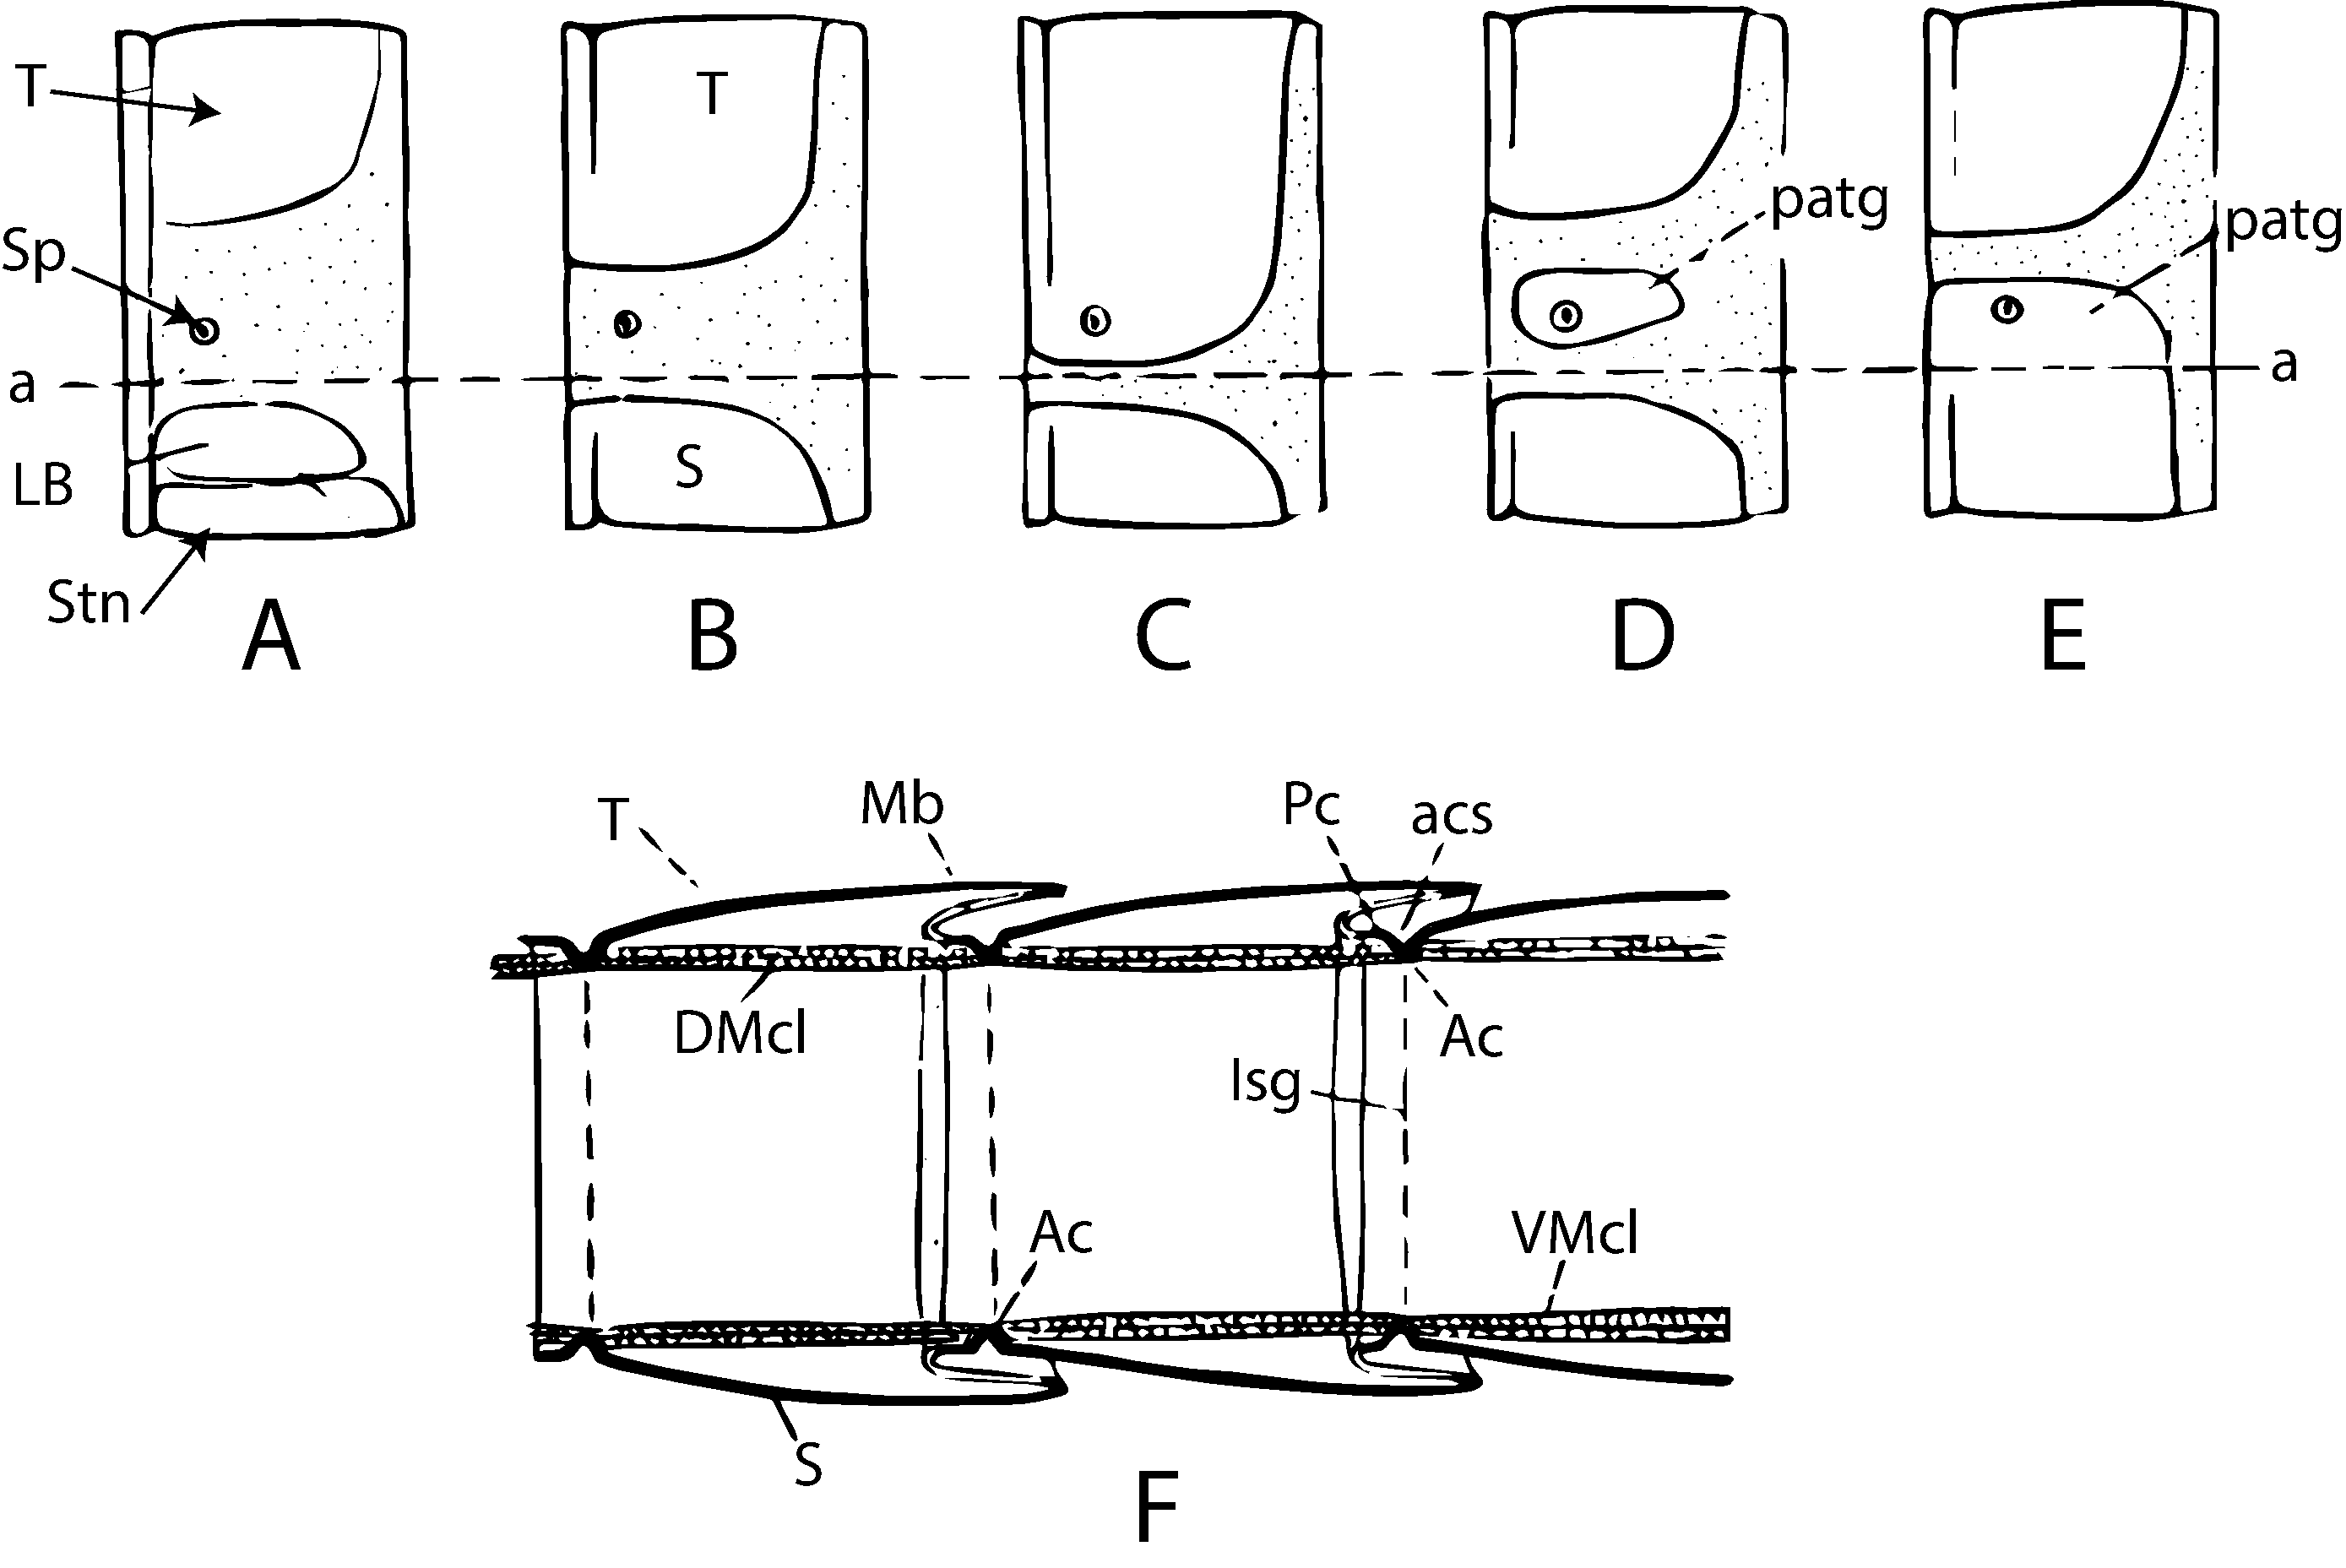
\includegraphics[width=0.7\textwidth]{morphology/abdomenSclerites}
  \caption{Abdominal sclerites. \citep[][Figs. 2A--F]{snodgrass1937morphology}}
  \label{fig:abdominalsclerites}
\end{figure}

\begin{figure}[ht!]
  \centering
    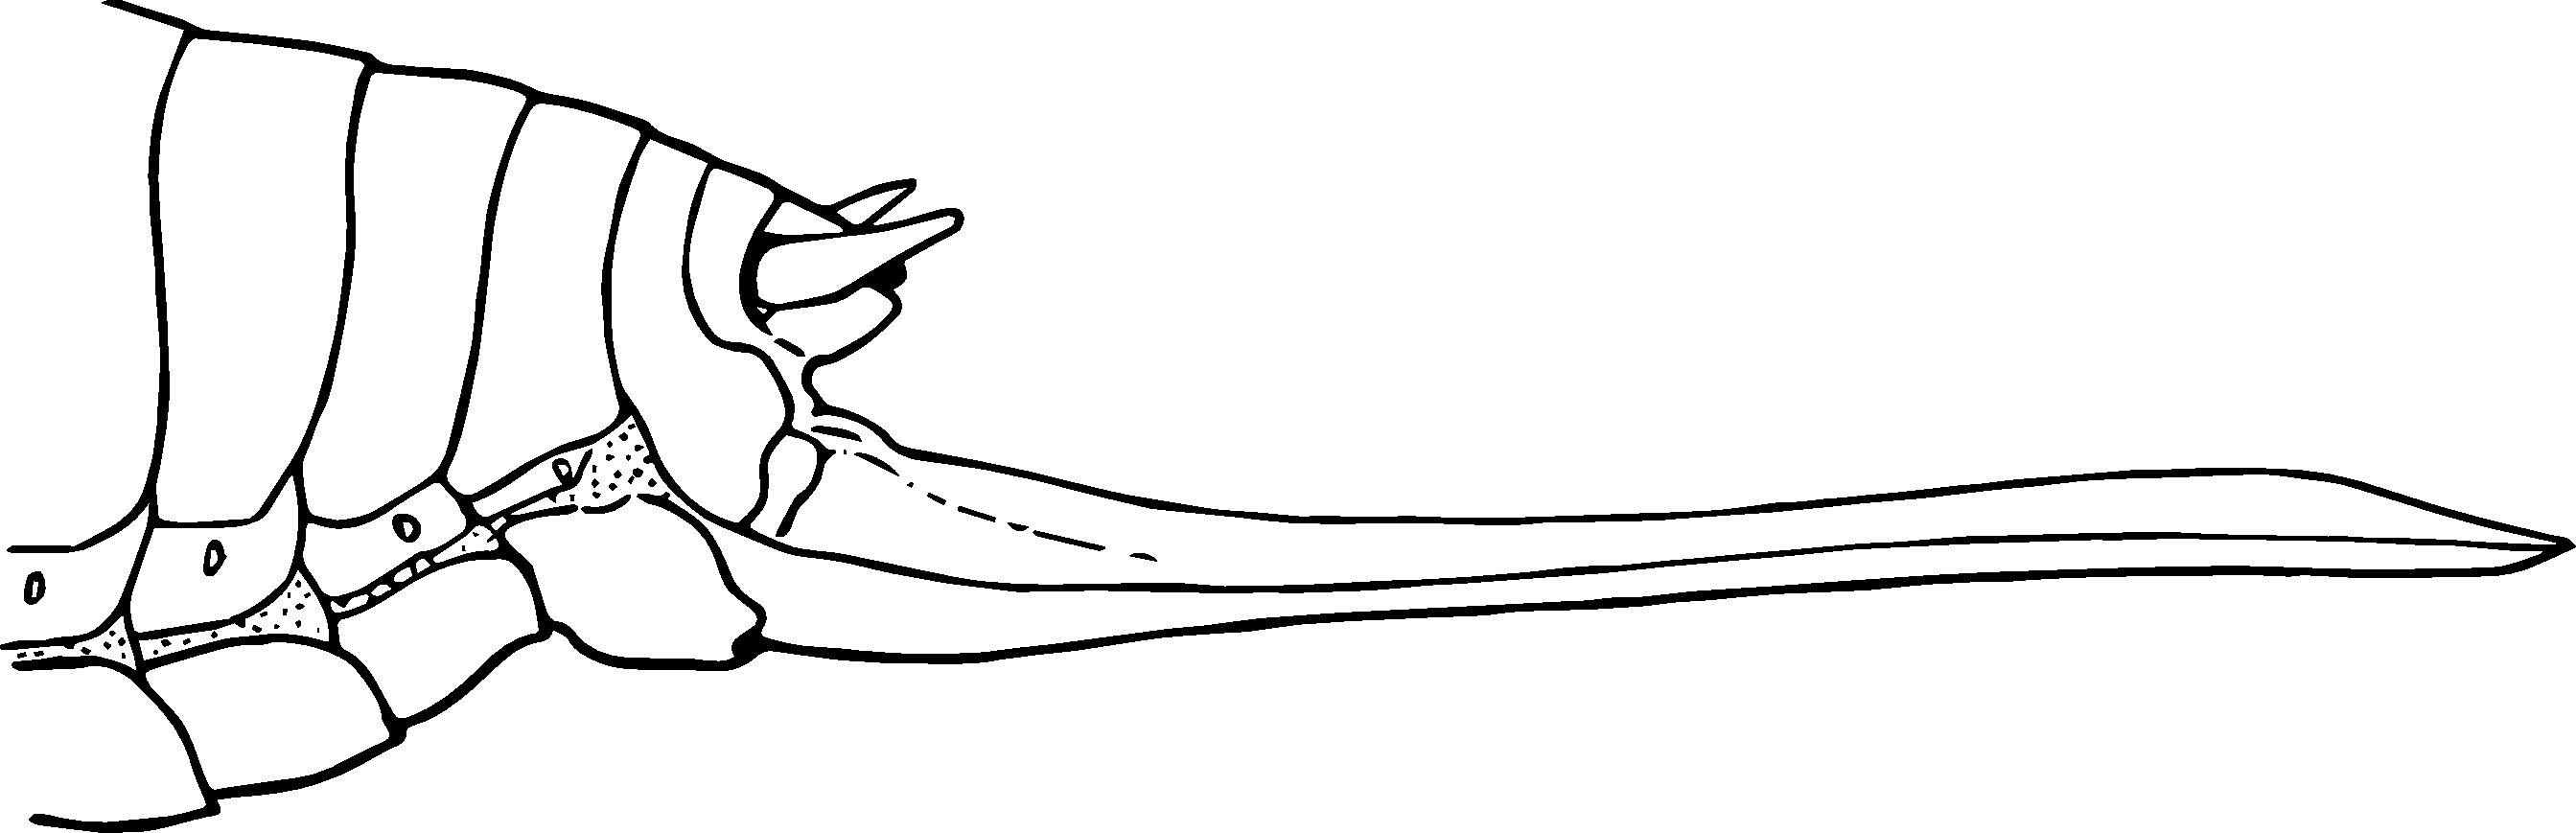
\includegraphics[width=0.7\textwidth]{morphology/ovipositor}
  \caption{Apex of female abdomen. \citep[][Fig. 74A]{bhl128276}}
  \label{fig:ovipositor}
\end{figure}

\noindent{}You should be able to see \latinword{spiracles} clearly on the abdomens of most insects. In most insects there are two sets of spiracles also on the thorax. Try to locate them in your winged arthropods, and then count the number of spiracles on the abdomen. Note that the second spiracle on the thorax is often difficult to find because it is located at the wing base.\vspace{3mm}

\begin{theo} 
{}Why is the abdomen generally softer and more flexible than the other tagmata? Why do we pin insects through the thorax?\end{theo}

\section{Cuticular features}

\noindent{}Select a specimen to examine under the microscope; a beetle would be good for this purpose. You should see hair-like cuticular modifications, \latinword{setae} (\latinword{seta}, sing.), which usually serve mechanosensory function. Sometimes these are modified as \latinword{scales}---\textit{i.e.}, they are flattened---which can also serve to present certain colors. If you look carefully you may also find other cuticular modifications: sensilla (\latinword{sensillum}, sing.), which usually look like pits or hairs, and pores. We will clarify the difference between \latinword{spurs} and \latinword{spines}.\\

\noindent{}Annotate the diagram below with each of the terms we discussed as a group.

\begin{figure}[ht!]
  \centering
    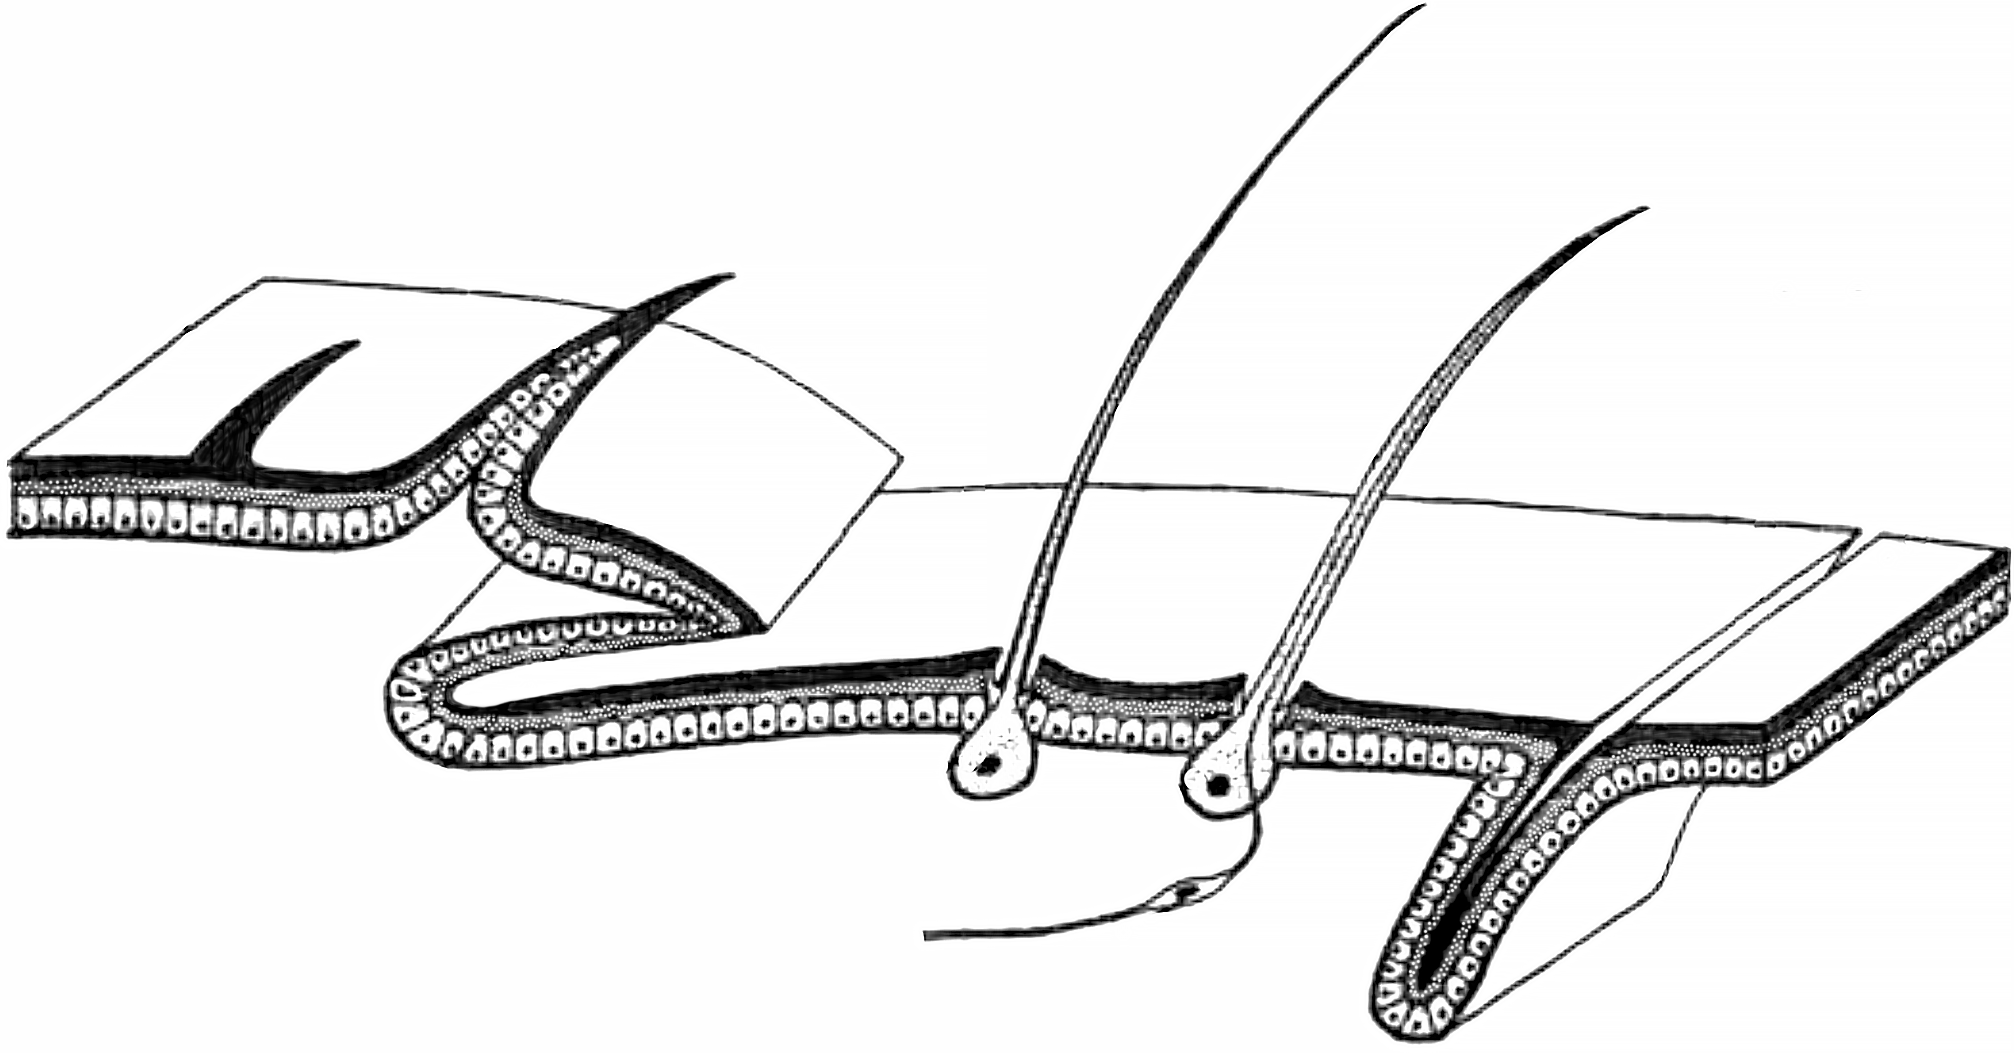
\includegraphics[width=0.7\textwidth]{morphology/cuticular}
  \caption{Features of insect cuticle \citep[redrawn and modified from][Fig. 43, a figure after illustrations by Snodgrass and Comstock]{metcalf1939destructive}}
  \label{fig:cuticular}
\end{figure}
\clearpage
\thispagestyle{empty}
